\usetikzlibrary{calc}
\usetikzlibrary{shapes,arrows}
%% ***********************************************************************
%\textsc{Reinforcement Learning and Dynamic Programming \hfill Spring 2014$\;$ \\
%Lecture Notes \hfill Shie Mannor and Nahum Shimkin \\
%\hfill Scribed by Michal Zarrouk}
%\vspace{-18pt}
%\par
%\hrulefill
%% ***********************************************************************
%
%% {\large
%
%

% \newcommand{\weights}{\texttt{w}}
\newcommand{\ftrs}{\phi}
\newcommand{\FtrMtx}{\Phi}

This chapter starts looking at the case where the MDP is
large. In the current chapter we will look at approximating the
value function. In the next chapter we will consider learning
directly a policy and optimizing it.

When we talk about a large MDP, it can be due to a few different
reasons. The most common is having a large state space $\States$. For example,
Backgammon has over $10^{20}$ states, Go has over $10^{170}$, and robot control typically 
has a continuous state space. The \textit{curse of dimensionality} is a common term for this problem, and relates to states that are composed of several state variables. For example, the configuration of a robot manipulator with $N$ joints can be described using $N$ variables for the angles at each joint. Assuming that each variable can take on $M$ different values, the size of the state space, $M^N$, grows exponentially with the number of state variables $N$.

Another reason why an MDP can be large is the size of the action space $\Actions$,
which can even be continuous in some applications (say, robots).
Finally, we might have complex dynamics $\transitionkernel$ that are hard to describe
succinctly (e.g., the next state is the result of a complex simulation) or are not even known to sufficient accuracy. 

Recall Bellman's dynamic programming equation,
$$\Value(\state) = \max_{\action \in \Actions} \left\{\reward(\state,\action) + \gamma \sum_{\state' \in \States} \transitionprob(\state'|\state,\action)\Value(\state')\right\}\quad \forall \state \in \States.$$
Dynamic programming requires knowing the model transitions $\transitionkernel$ and is only feasible for small problems, where iterating over all states and actions is feasible. The model-free and model-based learning algorithms described in Chapters \ref{chapter:learning-model-free} and \ref{chapter-model-based} do not require knowing the model, but require storing either value estimates \textit{for each} state and action, or state transition probabilities for every possible state, action, and next state. Scaling up our planning and RL algorithms to very large state and action spaces is the challenge we shall address in this chapter.


\section{Approximation approaches}
There are 4 main approaches for handling large MDPs:
\begin{enumerate}
\item \textbf{Myopic}: When $\transitionprob(\state'|\state,\action)$ is approximately uniform across $\action$ (that is, the actions do not have much effect on the transition to the next state), we may ignore the state transitions and simply use $\policy(\state)\approx \underset{\action \in \Actions}{\operatorname{argmax}} \{\reward(\state,\action)\}$. If $\reward(\state,\action)$ is not known exactly -- replace it with an estimate.

\item \textbf{Lookahead policies}: also known as rolling horizon/model-predictive control.\\
At each step $\ttime$, observe the state $\state_\ttime$ and simulate a horizon of $\tHorizon$ steps to calculate
$$\policy = \underset{\policy' \in \Policies}{\operatorname{argmax}}\  \mathbb{E}^{\policy'} \left[\left.\sum_{\ttime'=\ttime}^{\ttime+\tHorizon} \reward(\state_{\ttime'},\action_{\ttime'})\right|\state_\ttime\right].$$
Then, apply action $\policy(\state_\ttime)$, observe the resulting state transition to $\state_{\ttime+1}$, and repeat.

\item \textbf{Policy function approximation}\\
Assume the policy is of some parametric form $\policy(\state) = \policy(\state; \weight), \ \ \weight \in \mathtt{W}$, and optimize over parameters $\weight$.\\

\item \textbf{Value function approximation}\\
Assume the value function is of some parametric form and optimize over parameters $\weight$; the current chapter focuses on this approach.
When considering a value function approximation, there are a few interpretations
of what exactly we mean. Given a policy $\policy$, it can either be: (1) mapping from a state
$\state$ to its expected return, i.e.,
$\widehat{\Value}^\policy(\state;\weight)$. (2) mapping from state-action
pairs $(\state,\action)$ to their expected return, i.e.,
$\widehat{Q}^\policy(\state,\action;\weight)$. (3) mapping from
states $\state$ to expected return of each action, i.e.,
$\{\widehat{Q}^\policy(\state,\action_i;\weight):\action_i\in
\Actions\}$. All the interpretations are valid, and our
discussion will not distinguish between them (actually, for
$\{\widehat{Q}^\policy(\state,\action_i;\weight):\action_i\in
\Actions\}$ we implicitly assume that the number of actions is
small). We shall also be interested in approximating the optimal value function, and the corresponding approximations are denoted $\widehat{\Value}^*(\state;\weight)$, $\widehat{Q}^*(\state,\action;\weight)$, and $\{\widehat{Q}^*(\state,\action_i;\weight):\action_i\in
\Actions\}$, respectively.\\
Given an approximate $\widehat{Q}^*(\state,\action;\weight)$, we can derive an approximately optimal policy by choosing the \emph{greedy} action with respect to $\widehat{Q}^*(\state,\action;\weight)$.
\end{enumerate}

The 4 approaches above for dealing with large MDPs are not mutually exclusive and in practice, combining different approaches often produces the best performance. For example, a common approach is to combine a $\tHorizon$ step lookahead with an approximate terminal value function, 
\begin{equation*}
    \policy(\state_\ttime) = \underset{\pi' \in \Pi}{\operatorname{argmax}}\  \mathbb{E}^{\policy'} \left[\sum_{\ttime'=\ttime}^{\ttime+\tHorizon-1} \reward(\state_{\ttime'}) + \widehat{\Value}^*(\state_{\ttime+\tHorizon}))\right].
\end{equation*}
We shall also see, in the next chapter, that value function approximations will be a useful component in approximate policy optimization. In the rest of this chapter, we focus on value function approximation. 
We will consider (mainly) the discounted return with
a discount parameter $\gamma\in(0,1)$. The results extend 
naturally to the finite horizon and episodic settings.

% \tikzstyle{block} = [rectangle, draw,
%     text width=7em, text centered, rounded corners, minimum height=4em]
% \tikzstyle{blocks} = [rectangle, draw,
%     text width=4em, text centered, rounded corners, minimum height=4em]
% \tikzstyle{lblock} = [rectangle, draw,
%     text width=17em, text centered, rounded corners, minimum height=4em]
% \tikzstyle{line} = [draw, -latex']
% \begin{tikzpicture}[node distance = 1cm, auto]
%     % Place nodes
% %    \node [blocks] (a) {Chess game model};
%     \node [block] (b) {Feature extraction\\$\ftrs_1(s),...,\ftrs_k(s)$};
%     \node [block, right of = b, node distance=1.3in] (c) {Compute value\\function weights\\$\weight_1,...,\weight_k$};
%     \node [block, right of = c, node distance=1.3in] (d) {Set\\ $\widehat{\Value}^*(\state;\weight)$};
%     \node [lblock, right of = d, node distance=2.1in] (e) {\small$\policy(\state_\ttime) = \underset{\pi' \in \Pi}{\operatorname{argmax}}\  \mathbb{E}^{\policy'} \left[\sum_{\ttime'=\ttime}^{\ttime+\tHorizon-1} \reward(\state_{\ttime'}) + \widehat{\Value}^*(\state_{\ttime+\tHorizon}))\right]$};
%     % Draw edges
% %    \path [line] (a) -- (b);
%     \path [line] (b) -- (c);
%     \path [line] (c) -- (d);
%     \path [line] (d) -- (e);
% \end{tikzpicture}

\subsection{Value Function Approximation Architectures}\label{ssec:value_func_approx_arch}

We now discuss how to build the approximating function. For this we can consider popular hypothesis classes from the machine learning literature. 
For example: (1) Linear
functions, (2) Neural networks, (3) Decision trees, (4) Nearest
neighbors, (5) Fourier or wavelet basis, etc. We will concentrate
here on linear functions.
% and neural networks, mainly since gradient based methods apply to them very naturally.

In a linear function approximation, we represent the value as a weighted combination of some $\nftrs$ features:
$$\widehat{\Value}^\policy(\state;\weight) = \sum_{j=1}^\nftrs \weight_j \ftrs_j(\state) = \weight^T \ftrs(\state),$$
where $\weight \in \mathbb{R}^\nftrs$ are the function approximation parameters and $\ftrs(\state) \in \mathbb{R}^\nftrs$ are the states' \emph{features} (a.k.a. basis functions). Similarly, for state-action value functions, we use state-action features, $\ftrs(\state,\action)\in \mathbb{R}^\nftrs$, and approximate the value by $\widehat{Q}^\policy(\state,\action;\weight) =  \weight^T \ftrs(\state,\action)$.

Popular examples of state feature vectors include radial basis functions $\phi_j(\state) \propto \exp(\frac{(\state-\mu_j)^2}{\sigma_j})$, and tile features, where $\phi_j(\state) = 1$ for a set of states $A_j \subset \States$, and $\phi_j(\state) = 0$ otherwise. For state-action features, when the number of actions is finite $\Actions = \left\{1,2,\dots,|\Actions|\right\}$, a common approach is to extend the state features independently for every action. That is, consider the following construction for $\ftrs(\state,i)\in \mathbb{R}^{\nftrs \cdot |\Actions|}$, $i\in \Actions$:
\begin{equation*}
    \ftrs(\state,i)^T = \left[ \underbrace{\mathbf{0}^T, \mathbf{0}^T, \dots, \mathbf{0}^T}_{i-1 \text{ times}}, \ftrs(\state)^T, \underbrace{\mathbf{0}^T, \dots, \mathbf{0}^T}_{|\Actions|-i \text{ times}}\right],
\end{equation*}
where $\mathbf{0}$ is a vector of $\nftrs$ zeros.

However, for most interesting settings designing appropriate features is a difficult problem that requires significant domain knowledge. In the following, we assume that the features $\ftrs(\state)$ (or $\ftrs(\state,\action)$) are given to us in advance, and we concentrate on general methods for learning weights $\weight$ that minimize the approximation error as best as possible, with respect to the available features. 

\section{Quantification of Approximation Error}

Before we start the discussion on learning methods, we take a small detour to discuss the effect of error in the value function. Assume we
have a value function $\widehat{\Value}$ such that $\|\widehat{\Value}-\Value^*\|_\infty\leq
\varepsilon$. Let $\widehat{\policy}$ be the greedy policy with respect to
$\widehat{\Value}$, namely,
\[
\widehat{\policy}(\state)=\arg\max_\action [\reward(\state,\action)+\gamma
\mathbb{E}_{\state'\sim \transitionprob(\cdot|\state,\action)}[\widehat{\Value}(\state')]].
\]


\begin{theorem}\label{thm:approx_error}
Let $\widehat{\Value}$ such that $\|\widehat{\Value}-\Value^*\|_\infty\leq \varepsilon$ and
$\widehat{\policy}$ be the greedy policy with respect to $\widehat{\Value}$. Then,
\[
\|\Value^{\widehat{\policy}}-\Value^*\|_\infty\leq\frac{2\gamma\varepsilon}{1-\gamma}.
\]
\end{theorem}

\begin{proof}
Consider two operators $\operator^\policy$ and $\operator^*$ (see
Chapter \ref{ss:DP_op}). The first, $\operator^\policy$, is
\[
(\operator^\policy v)(\state)=\reward(\state,\policy(\state))+\gamma
\mathbb{E}_{\state'\sim \transitionprob(\cdot|\state,\policy(\state))}[v(\state')],
\]
and it converges to $\Value^\policy$ (see Theorem~\ref{thm:DP_op}).
The second, $\operator^*$, is
\[
(\operator^* v)(\state)=\max_\action[\reward(\state,\action)+\gamma
\mathbb{E}_{\state'\sim \transitionprob(\cdot|\state,\action)}[v(\state')] ],
\]
and it converges to $\Value^*$ (see Theorem~\ref{thm:DP_op}).
In addition, we have shown that both
$\operator^\policy$ and $\operator^*$ are $\gamma$-contracting (see
Theorem~\ref{thm:DP_op}).

Since $\widehat{\policy}$ is greedy with respect to $\widehat{\Value}$ we have
$\operator^{\widehat{\policy}} \widehat{\Value}=\operator^* \widehat{\Value}$ (but this does not hold for
other value functions $\Value' \neq \widehat{\Value}$).

Then,
\begin{align*}
\|\Value^{\widehat{\policy}}-\Value^*\|_\infty &= \|\operator^{\widehat{\policy}} \Value^{\widehat{\policy}} - \Value^*\|_\infty\\
&\leq \|\operator^{\widehat{\policy}} \Value^{\widehat{\policy}} -\operator^{\widehat{\policy}} \widehat{\Value}\|_\infty +\|\operator^{\widehat{\policy}} \widehat{\Value} - \Value^*\|_\infty\\
&\leq \gamma\| \Value^{\widehat{\policy}} - \widehat{\Value}\|_\infty +\|\operator^* \widehat{\Value} - \operator^*\Value^*\|_\infty\\
&\leq \gamma\| \Value^{\widehat{\policy}} - \widehat{\Value}\|_\infty +\gamma\| \widehat{\Value} - \Value^*\|_\infty\\
&\leq \gamma(\| \Value^{\widehat{\policy}} - \Value^*\|_\infty+ \|\Value^*-\widehat{\Value}\|_\infty ) +\gamma\| \widehat{\Value} - \Value^*\|_\infty\;,
\end{align*}
where in the second inequality we used the fact that since since
$\policy$ is greedy with respect to $\widehat{\Value}$ then $\operator^{\widehat{\policy}} \widehat{\Value}=\operator^* \widehat{\Value}$.

Reorganizing the inequality and recalling that
$\|\Value^*-\widehat{\Value}\|_\infty\leq \varepsilon$, we have
\[
(1-\gamma)\|\Value^{\widehat{\policy}}-\Value^*\|_\infty \leq 2\varepsilon\gamma,
\]
and the theorem follows.
\end{proof}

The above theorem states that if we have small errors in
$L_\infty$ norm, the effect of the errors on the expected return is
bounded. However, in most cases we will not be able to guarantee an
approximation in norm $L_\infty$. In fact, even if $\Value^*$ is given to us, it is infeasible to compute $\|\Value^{\widehat{\policy}}-\Value^*\|_\infty$ in the large state space setting, as it requires iterating over \textit{all} states. 

Intuitively, a more feasible guarantee is that some \textit{average} error is small. In the following, we shall see that this condition can be represented mathematically as a weighted $L_2$ norm. Extending Theorem \ref{thm:approx_error} to a weighted $L_2$ norm is possible, but is technically involved~\cite{munos2007performance}, and we will not derive it in this book. Nevertheless, we shall next study learning algorithms that have a guaranteed average error bound.

\section{Approximate Policy Evaluation}\label{sec:approx_policy_eval}

We begin our investigation with the problem of approximating the value function of a given policy. We shall later discuss methods that improve a policy, or approximate the optimal value function.


\subsection{From RL to Supervised Learning}

To learn the value function, we would like to reduce our reinforcement learning problem to a
supervised learning problem. This will enable us to use any of the many techniques of machine learning to address the problem. Let us consider the basic ingredients of supervised learning. The first ingredient is a labeled training set that is sampled i.i.d.

Let us start by considering an idealized setting. Fix a policy $\policy$, and consider learning its value function $\widehat{\Value}^{\policy}$. To apply supervised learning, we should
generate a training set, i.e., 
\[
\{(\state_1, \Value^\policy(\state_1)),\ldots,
(\state_m,\Value^\policy(\state_m))\},
\]
where $\Value^\policy(\state))$ is the label of a sample state $\state$.

We first need to discuss how to sample the states $\state_i$ in an
i.i.d. way. We can generate a trajectory, but we need to be careful,
since adjacent states are definitely dependent! One solution is to
space the sampling from the trajectory using the mixing time of
$\policy$.\footnote{See Chapter \ref{chapter:MC} for definition.}
This will give us samples $\state_i$ which are sampled (almost) from the
stationary distribution of $\policy$ and are (almost) independent. In the episodic setting, we can sample different episodes, and states from different episodes are guaranteed to be independent.
%For the action, we clearly will use $\policy$, no problem there.

Second, we need to define a loss function, which will tradeoff the different approximation errors. Since the value is a real scalar, a natural candidate is the average squared error loss, $\frac{1}{m}\sum_{i=1}^m (\widehat{\Value}^\policy(\state_i) - \Value^\policy(\state_i))^2$. With this loss, the corresponding supervised learning problem is least squares regression.

The hardest, and most confusing, ingredient is generating the labels
$\Value^\policy(\state_i)$. In supervised machine leaning we assume
that someone gives us the labels to build a classifier.
% (or alternatively, in unsupervised learning, where there is no clear ground truth).
However, in our problem, the value function is exactly what we want to learn, and it is not realistic to assume any ground truth samples from it!

Our main task, therefore, would be to replace the ground truth labels with quantities that we can measure, using simulation or interaction with the system. We shall start by formally defining least squares regression in a way that will be convenient to extend later to RL.



% \section{Approximation Methods in Value Space}
% \begin{enumerate}
% \item Approximate policy iteration: approximate $\Value^\policy$; improve $\policy$; repeat.
% \item Approximate value iteration / Q-learning: $\widehat{Q}(s,a)\approx {\ftrs}(s,a)^\top {\weight}$
% % \item Bellman error minimization:
% % $$ \min_\weights \  \mathbb{E}_s \left[\left(\tilde{V}(s;\weights)-T\tilde{V}(s;\weights)\right)^2\right]$$
% % where $T$ is the Bellman operator and $\mathbb{E}_s$ is w.r.t. some distribution over the states.
% \item Linear programming: not discussed.
% \end{enumerate}

% Note that both $V$ and $Q$ are mappings from a state (or state-action) to $\mathbb{R}$. When the state space is large, we will not be able to calculate the value for every state, but instead, fit an approximate function based on a few states for which their values can be calculated (or estimated). This is similar to a \emph{regression} problem, which our development will be based on, but as we shall see, we will also need to account for the dynamic nature of the problem to develop approximate optimization algorithms.

% \subsection{Approximate Policy Evaluation}

% We start with the simplest setting - approximating the value of a fixed policy. A direct approach for this task is through regression, which we will now review. 

\subsection{Preliminaries -- Least Squares Regression}\label{ssec:least_squares_regression}
To simplify our formulation, we will assume that the state space may be very large, but finite. Equivalently, we will consider a regression problem where the independent variable can only take a finite set of values. 

Assume we have some function $y = f(x)$, where $y \in \mathbb{R}$, $x\in X$, and $X$ is finite. As usual, $x$ is termed the independent variable, while $y$ is the dependent variable. We assume that data is generated by sampling i.i.d. from a distribution $\xi(x)$, and the labels are noisy. That is, we are given $N$ labeled samples $\left\{(x_1, y_1),\dots, (x_N, y_N) \right\}$, where $x_i \sim \xi(x)$, $y_i = f(x_i) + \omega(x_i)$, and $\omega(x)$ is a zero-mean i.i.d. noise (which may depend on the state).

Our goal is to fit to our data a parametric function $g(x;\weights):X \to \mathbb{R}$, where $\weights \in \mathbb{R}^{\nftrs}$, such that $g$ approximates $f$ well. The Least Squares approach solves the following problem:
\begin{equation}\label{eq:least_squares}
\hat{\weights}_{LS} = \min_\weights \frac{1}{N}\sum_{i=1}^N (g(x_i;\weights) - y_i)^2.
\end{equation}
A practical iterative algorithm for solving \eqref{eq:least_squares} is the stochastic gradient descent (SGD) method, which updates the parameters by
\begin{equation}\label{eq:sgd}
\weights_{i+1} = \weights_i - \alpha_i (g(x_i;\weights_i) - y_i)\nabla_\weights g(x_i;\weights_i),
\end{equation}
where $\alpha_i$ is some step size schedule, such as $\alpha_i = 1/i$.
% $$
% \min_\weights \mathbb{E}_{x\sim\xi} (g(x;\weights) - f(x))^2.
% $$



When $g$ is linear in some features $\ftrs(x)$, i.e., $g(x;\weights) = \weights^T \ftrs(x)$, the least squares solution can be calculated explicitly. Let $\hat{\FtrMtx} \in \mathbb{R}^{N \times \nftrs}$ be a matrix with $\ftrs(x_i)$ in its rows, often called the \textit{design matrix}. Similarly, let $\hat{Y}\in \mathbb{R}^{N \times 1}$ be a vector of $y_i$'s. Then, Equation \eqref{eq:least_squares} can be written as
\begin{equation}\label{eq:linear_least_squares}
\hat{\weights}_{LS} = \min_\weights \frac{1}{N} (\hat{\FtrMtx} \weights - \hat{Y})^T(\hat{\FtrMtx} \weights - \hat{Y}) = 
\min_\weights \frac{1}{N} \left( \weights^T (\hat{\FtrMtx}^T \hat{\FtrMtx}) \weights -2 \weights^T \hat{\FtrMtx}^T \hat{Y} + \hat{Y}^T\hat{Y} \right).
\end{equation}
Noting that \eqref{eq:linear_least_squares} is a quadratic form, the least squares solution is: 
\begin{equation}\label{eq:sampled_LS}
    \hat{\weights}_{LS} = (\hat{\FtrMtx}^T \hat{\FtrMtx})^{-1} \hat{\FtrMtx}^T \hat{Y}.
\end{equation}

We now show that the LS solution \eqref{eq:sampled_LS} converges to the \textit{expected} least squares solution when $N \to \infty$.
Without loss of generality, we assume that the states are ordered, $1,2,\dots,|X|$. Let $\xi\in \mathbb{R}^{|X|}$ denote a vector of probabilities for each state $\xi(x)$, and define the diagonal matrix
$\Xi = \text{diag}(\xi)\in\mathbb{R}^{|X| \times |X|}$. Further, let $\FtrMtx \in \mathbb{R}^{|X| \times \nftrs}$ be a matrix with $\ftrs(x)$ as its rows, and let $Y\in \mathbb{R}^{|X|}$ be a vector of $f(x)$.


\begin{proposition}
Assume that $\FtrMtx^T \Xi \FtrMtx$ is not singular (i.e., no feature is a linear combination of other features and each state has a positive probability). Then $\lim_{N \to \infty} \hat{\weights}_{LS} = \weights_{LS}$, where
\begin{equation*}
    \weights_{LS} = (\FtrMtx^T \Xi \FtrMtx)^{-1} \FtrMtx^T \Xi Y.
\end{equation*}
\end{proposition}

\begin{proof}
From the law of large numbers, we have that 
\begin{equation*}
\begin{split}
    \lim_{N \to \infty}\frac{1}{N}\hat{\FtrMtx}^T \hat{\FtrMtx} &= \lim_{N \to \infty}\frac{1}{N} \sum_{i=1}^N \phi(x_i) \phi(x_i)^T \\
    &= \mathbb{E}_{x \sim \xi(x)}\left[ \phi(x) \phi(x)^T \right] \\
    &= \sum_{x} \xi(x) \phi(x) \phi(x)^T \\
    &= \FtrMtx^T \Xi \FtrMtx.
\end{split}
\end{equation*}
Similarly, $\lim_{N \to \infty}\frac{1}{N} \hat{\FtrMtx}^T \hat{Y} = \FtrMtx^T \Xi Y$. Plugging into Eq.~\eqref{eq:sampled_LS} completes the proof.
\end{proof}

Using the stochastic approximation technique, a similar result holds for the SGD update.
\begin{proposition}
Consider the SGD update in Eq.~\eqref{eq:sgd} with linear features, 
$$
\weights_{i+1} = \weights_i - \alpha_i ( \weights^T \ftrs(x_i) - y_i)\ftrs(x_i).
$$
Assume that $\FtrMtx^T \Xi \FtrMtx$ is not singular, and that the step sizes satisfy $\sum_i \alpha_i = \infty$ and $\sum_i \alpha_i^2 < \infty$. Then $\weights_{i} \to \weights_{LS}$ almost surely. 
\end{proposition}

Note that the expected LS solution can also be written as the solution to the following \textit{expected least squares} problem:
\begin{equation}\label{eq:LS_expected}
\weights_{LS} = \min_\weights (\FtrMtx \weights - Y)^T \Xi (\FtrMtx \weights - Y).
\end{equation}
Observe that $\FtrMtx \weights_{LS} \in \mathbb{R}^{|X|}$ denotes a vector that contains the approximated function $g(x;\weights_{LS})$ for every $x$. 
This is the best approximation of $f$ in the span of the features $\ftrs(x)$, in terms of expected square error. Recalling that $Y$ is a vector of ground truth $f$ values, we view this approximation as a \emph{projection} of $Y$ onto the space spanned by $\FtrMtx \weights$, and we can write the projection operator explicitly as:
$$
\Project_\xi Y = \FtrMtx \weights_{LS} = \FtrMtx (\FtrMtx^T \Xi \FtrMtx)^{-1} \FtrMtx^T \Xi Y.
$$

Geometrically, $\Project_\xi Y$ is the vector that is closest to $Y$ on the linear subspace $\FtrMtx \weights$, where the distance function is the $\xi$-weighted Euclidean norm, $||z||_\xi = \sqrt{\langle z,z\rangle_\xi}$, where $\left\langle z, z' \right \rangle_\xi = z^T \Xi z'$.

We conclude this discussion by noting that although we derived Eq.~\eqref{eq:LS_expected} as the expectation of the least square method, we could also take an alternative view: the least squares method in \eqref{eq:sampled_LS} and the SGD algorithm are two different \textit{sampling} based approximations to the expected least squares solution in \eqref{eq:LS_expected}. We will take this view when we develop our RL algorithms later on.

% In the non-linear case, a common approach is to solve the least squares problem by gradient descent, i.e., $\weights_{k+1} = \weights_k - \alpha_k \nabla_\weights \mathbb{E}_{x\sim\xi} (g(x;\weights) - f(x))^2,$ where the gradient is simply $2 \mathbb{E}_{x\sim\xi} (g(x;\weights) - f(x))\nabla_\weights g(x;\weights)$. 

% In a practical case, we are given $N$ data samples $\{ x_i, y_i \}: x_i\sim \xi, y_i=f(x_i)$. The least squares solution can be approximated from the samples as:
% $$
% \min_\weights \sum_i (g(x_i;\weights) - y_i)^2,
% $$
% The stochastic gradient descent (SGD) version of this update is
% $$
% \weights_{k+1} = \weights_k - \alpha_k (g(x_i;\weights_k) - y_i)\nabla_\weights g(x_i;\weights_k).
% $$

% For the linear case, we can solve directly:
% $$
% \hat{\weights}_{LS} = (\hat{\FtrMtx}^T \hat{\FtrMtx})^{-1} \hat{\FtrMtx}^T \hat{Y},
% $$
% where in this case the rows of $\hat{\FtrMtx}$ and $\hat{Y}$ are given by the $N$ samples. By the law of large numbers, we have that $\frac{1}{N}(\hat{\FtrMtx}^T \hat{\FtrMtx}) \to (\FtrMtx^T \Xi \FtrMtx)$ and $\frac{1}{N}\hat{\FtrMtx}^T \hat{Y} \to \FtrMtx^T \Xi Y$, thus the sampled solution converges to the solution $\weights_{LS}$ above.

\subsection{Approximate Policy Evaluation: Regression}

We now consider the simplest value function approximation method -- regression, also known as Monte Carlo (MC) sampling. Recall that we are interested in learning the value function of a fixed policy $\policy$, $\widehat{\Value}^{\policy}$.
Based on the least squares method above, all we need to figure out is how to build the sample, namely, how do we set the labels to
replace $\Value^\policy (\state)$. The basic idea is to find an
unbiased estimator $U_\ttime$ such that $E[U_\ttime
|\state_\ttime]=\Value^\policy(\state_\ttime)$. The Monte-Carlo (MC) estimate, which was introduced in Chapter \ref{sec:MC}, simply sums the observed discounted reward from a state $R_\ttime(\state)=\sum_{\tau=0}^T
\discount^\tau \reward_\tau$, starting at the first visit of $\state$ in episode
$\ttime$. Clearly, we have
$E[R_\ttime(\state)]=\Value^\policy(\state)$, since samples are
independent, so we can set $U_\ttime(\state)=R_\ttime(\state)$. 


For calculating the approximation, we can apply the various least squares algorithms outlined above. In particular, for a linear approximation, and a large sample, we understand that the solution will approach the projection, $\FtrMtx \weights = \Project_\xi \Value^\policy$.
% The direct approach to policy evaluation: Evaluate $\Value^\policy(s)$ only for several states (e.g. by simulation) and interpolate, e.g., using least squares regression: $\FtrMtx \weights = \Project_\xi \Value^\policy$. This method is simple, however, it has several drawbacks. The first is that value estimates typically have a large variance, as they accumulate rewards from multiple states in the future. The second is that we need to wait for full simulations to complete before updating the value estimate. Practically, this can take too long in some problems. 

% We next describe an alternative approach, using the fact that the value function satisfies Bellman's equation.

\subsection{Approximate Policy Evaluation: Bootstrapping}\label{ssec:APE_bootstrapping}
While the MC estimate is intuitive, it turns out that there is a more efficient way of estimating labels for regression, based on the idea bootstrapping (cf. Chapter \ref{chapter:learning-model-free}). We motivate this approach with an example.

\begin{figure}
    \centering
    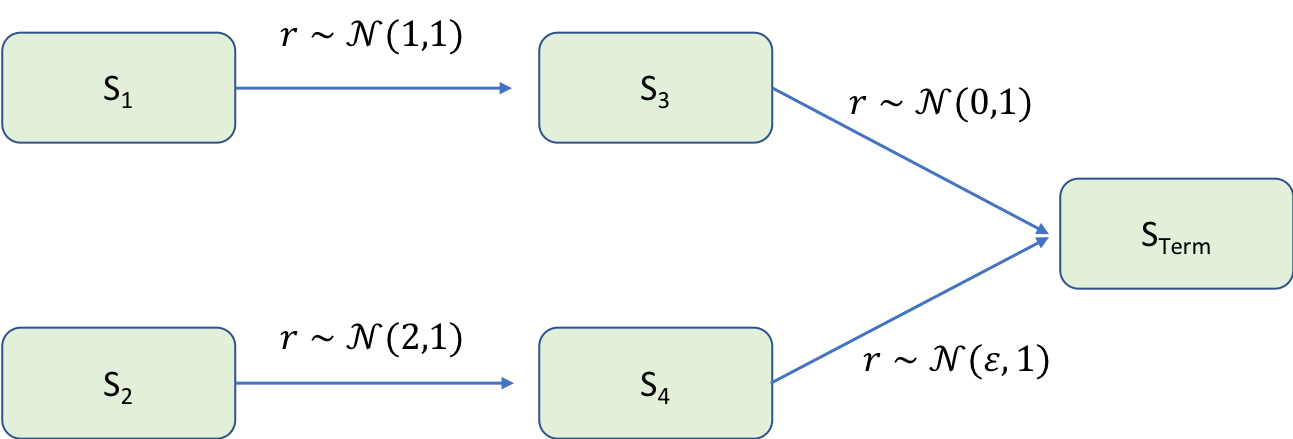
\includegraphics[width=\textwidth]{figures/td_vs_mc_FA.png}
    \caption{Example: MC vs. TD with function approximation.}
    \label{fig:td_vs_mc_FA}
\end{figure}

Consider the episodic MDP in Figure \ref{fig:td_vs_mc_FA}.
In this MDP there are two paths towards a terminal state. The first state in each path gives a large reward that determines most of the total return. The second state on each path gives a small reward that does not affect the total return by much, and therefore, the values of each of these second states are similar. We shall show that this value similarity may be exploited to reduce the variance in the estimates of the initial state values $\Value^{\policy}(\state_1)$ and $\Value^{\policy}(\state_2)$.

Formally, $\state_{Term}$ is a terminal state, and rewards are normally distributed with unit variance, as shown. There are no actions, and therefore for any $\policy$, $\Value^{\policy}(\state_1) = 1$, $\Value^{\policy}(\state_2) = 2+\varepsilon$, $\Value^{\policy}(\state_3) = 0$, and $\Value^{\policy}(\state_4) = \varepsilon$. We will particularly be interested in estimating $\Value^{\policy}(\state_1)$ and $\Value^{\policy}(\state_2)$.

Consider the case of no function approximation. Assume that we have sampled $N$ trajectories, where half start from $\state_1$, and the other half from $\state_2$. In this case, the MC estimates for $\widehat{\Value}^{\policy}(\state_1)$ and $\widehat{\Value}^{\policy}(\state_2)$ will each be based on $N/2$ samples, and their variance will therefore be $2 / ({N}/{2}) = 4/{N}$.

Let us recall the bootstrapping approach. We have that $\Value^{\policy}(\state_1) = \mathbb{E}\left[ \reward(\state_1)\right] + \Value^{\policy}(\state_3)$, and similarly, $\Value^{\policy}(\state_2) = \mathbb{E}\left[ \reward(\state_2)\right] + \Value^{\policy}(\state_4)$. Therefore, we can use the samples to first estimate $\widehat{\Value}^{\policy}(\state_3)$ and $\widehat{\Value}^{\policy}(\state_4)$, and then plug in to estimate $\widehat{\Value}^{\policy}(\state_1)$ and $\widehat{\Value}^{\policy}(\state_2)$.

Now, for small $\varepsilon$, we understand that the values $\Value^{\policy}(\state_3)$ and $\Value^{\policy}(\state_4)$ should be similar. One way to take this into account is to use function approximation that approximates $\Value^{\policy}(\state_3)$ and $\Value^{\policy}(\state_4)$ as \textit{the same} value, $\widehat{\Value}_{3/4}$. In this approximation we effectively use the full $N$ samples to estimate $\widehat{\Value}_{3/4}$, resulting in variance $1/{N}$. We can now use bootstrapping to estimate $\widehat{\Value}^{\policy}(\state_1)$ and $\widehat{\Value}^{\policy}(\state_2)$, which will result in variance $1 / {N}+ 1 / ({N}/{2}) = 3/{N}$, smaller than the MC estimate!

However, note that for $\varepsilon \neq 0$, the bootstrapping solution will also be biased: taking $N\to \infty$ we see that $\widehat{\Value}_{3/4}$ will converge to $\varepsilon/2$, and therefore $\widehat{\Value}^{\policy}(\state_1)$ and $\widehat{\Value}^{\policy}(\state_2)$ will converge to $1+\varepsilon/2$ and $2+\varepsilon/2$, respectively.

Thus, we see that bootstrapping, when combined with function approximation, allowed us to reduce variance by exploiting the similarity between values of different states, but at the cost of a possible bias in the expected solution. As it turns out, this phenomenon is not limited to the example above, but can be shown to hold more generally~\cite{kearns2000bias}. 
% \AT{I don't know of a general result about bias/variance that is simple enough to state in the book. Any ideas?}

In the following, we shall develop a rigorous formulation of bootstrapping with function approximation, and use it to suggest several approximation algorithms. We will also bound the bias incurred by this approach.

\subsection{Approximate Policy Evaluation: the Projected Bellman Equation}

% A key step in approximate policy iteration here is the policy evaluation: given $\policy$ we would like to approximate $\Value^\policy$. There are two main methods for approximate policy evaluation:
% \begin{enumerate}
% \item Direct approach: Evaluate $\Value^\policy(s)$ only for several states (e.g. by simulation) and interpolate, e.g., using least squares regression: $\FtrMtx \weights = \Pi \Value^\policy$. This method is simple, however, it has several drawbacks. The first is that value estimates typically have a large variance, as they accumulate rewards from multiple states in the future. The second is that we need to wait for full simulations to complete before updating the value estimate. Practically, this can take too long in some problems. 
% \item 
Recall from Chapter \ref{chapter:learning-model-free} that without function approximation, TD methods effectively compute a solution to the Bellman equation. With function approximation, this is no longer the case, as clearly  whatever solution TD methods converge to (if they converge at all), must depend on the function approximation. We shall start our investigation from a fundamental equation that takes function approximation into account -- the projected Bellman equation (PBE). We will use the PBE to define a particular approximation of the value function, and study its properties. We will later develop TD algorithms that estimate this approximation using sampling.

For technical simplicity, our analysis mainly considers linear function approximation. The algorithms we develop, however, can easily be extended to non-linear  approximation, and we will expand on particular cases where relevant. Let $\FtrMtx \in \mathbb{R}^{|\States|\times \nftrs}$ denote a matrix in which each row $\state$ is $\ftrs(\state)$, where without loss of generality we assume that the states are ordered as $1,2,\dots, |\States|$. 
Let $\ftrspace = \left\{ \FtrMtx \weights: \weights \in \mathbb{R}^{\nftrs} \right\}$ denote the linear subspace spanned by $\FtrMtx$.
Recall that $\Value^\policy(s)\in\mathbb{R}^{|\States|}$ satisfies the Bellman equation: $\Value^\policy = \operator^\policy \Value^\policy$. However, $\Value^\policy$ does not necessarily belong to $\ftrspace$, as we may not be able to accurately represent the true value function as a linear combination of our features. 

To write a `Bellman-like' equation that involves our function approximation, we proceed by projecting the Bellman operator $\operator^\policy$ onto $\ftrspace$, resulting in the PBE:
\begin{equation}\label{eq:PBE}
    \FtrMtx \weights = \Project_{\xi} \operator^\policy \{\FtrMtx \weights\},
\end{equation}
where $\Project_{\xi}$ is the projection operator onto $\ftrspace$ under some $\xi$-weighted Euclidean norm.

Let us try to intuitively interpret the PBE. We are looking for an approximate value function $\FtrMtx \weights \in \mathbb{R}^{|\States|}$, which by definition is within our linear approximation space, such that after we apply to it $\operator^\policy$, and project the result (which does not necessarily belong to $\ftrspace$ anymore) back to $\ftrspace$, we obtain the same approximate value. Since the true value is a fixed point of $\operator^\policy$, we have reason to believe that a fixed point of $\Project_{\xi}\operator^\policy$ may provide a reasonable approximation. In the following, we shall investigate this hypothesis, and build on Eq.~\eqref{eq:PBE} to develop various learning algorithms. We remark that the PBE is not the only way of defining an approximate value function, and other approaches have been proposed in the literature. However, the PBE is the basis for the most popular RL algorithms today.
    % \begin{equation*}
    %     \weights_k= \underset{\weights}{\operatorname{argmin}} \{||\FtrMtx \weights - T^{\policy_k}\FtrMtx \weights_k||_\xi^2\}.
    % \end{equation*}
% Includes:
% \begin{itemize}
% \item Temporal differences - TD(0): online solution of the PBE.
% % $\FtrMtx \weights = \Pi \operator^\policy \{\FtrMtx \weights\}$, where $\Pi$ is the projection operator onto $\mathcal{S}$ under some norm.\\
% \item Least-squares policy evaluation - LSPE(0): simulation-based form
% \begin{align*}\FtrMtx \weights_{k+1} = \Pi \operator^\policy \{\FtrMtx \weights_k\} + \mathrm{noise}.\end{align*} 
% \item Least-squares temporal differences - LSTD(0): batch solution of the PBE.
% \end{itemize}
% \end{enumerate}

% We now discuss the indirect approach to policy evaluation.

% Define the weighted Euclidean inner product:
% $$\langle V_1,V_2\rangle_\xi = {\sum_{i=1}^n \xi_i V_1(i)V_2(i)}, \ \ \xi_i\ge0,$$
% and the induced weighted Euclidean norm:
% $$||V||_\xi = \sqrt{\langle V,V\rangle_\xi} = \sqrt{\sum_{i=1}^n \xi_i V(i)^2}, \ \ \xi_i\ge0,$$
% and let $\Project_\xi$ be the operator of projection onto $\mathcal{S}$ w.r.t. this norm:
% \begin{align*}\Project_\xi V &=\underset{V' \in \mathcal{S}}{\operatorname{argmin}} \ ||V'-V||_\xi =\\
% &= \FtrMtx \weights \ \ \ \mathrm{s.t.} \ \ \weights = \underset{\weights' \in \mathbb{R}^k}{\operatorname{argmin}} \ ||\FtrMtx \weights' - V||_\xi.\end{align*}

% We want to solve the projected Bellman equation (PBE):
% \begin{equation}\label{eq:PBE}
% \FtrMtx \weights^*  = \Project_\xi \operator^\policy \FtrMtx \weights^*.
% \end{equation}
% The main reason to consider the approximation in \eqref{eq:PBE} is that, as we shall see, it will allow us to derive efficient sampling based algorithms with provable error guarantees.

\subsubsection{Existence, Uniqueness and Error Bound on PBE Solution}
We are interested in the following questions:
\begin{enumerate}
\item Does the PBE \eqref{eq:PBE} have a solution?
\item When is $\Project_\xi \operator^\policy$ a contraction, and what is its fixed point?
\item If $\Project_\xi \operator^\policy$ has a fixed point $\FtrMtx\weights^*$, how far is it from the best approximation possible, namely, $\Project_\xi  \Value^\policy$?
\end{enumerate}
Answering the first two points will characterize the approximate solution we seek. The third point above relates to the bias of the bootstrapping approach, as described in the example in Section \ref{ssec:APE_bootstrapping}. 

Let us assume the following:
\begin{assumption}\label{ass:recurrent}The Markov chain corresponding to $\policy$ has a single recurrent class and no transient states. We further let
$$\xi_j = \lim_{N\rightarrow \infty} \frac{1}{N} \sum_{\ttime=1}^N P(\state_\ttime=j|\state_0=\state)>0,$$
which is the probability of being in state $j$ when the process reaches its steady state, given any arbitrary $\state_0=\state$.
\end{assumption}
We have the following result:
\begin{proposition}\label{prop:PBE_contraction} Under Assumption \ref{ass:recurrent} we have that
\begin{enumerate}
\item $\Project_\xi \operator^\policy$ is a contraction operator with modulus $\gamma$ w.r.t. $||\cdot||_\xi$.
\item The unique fixed point $\FtrMtx \weights^*$ of $\Project_\xi \operator^\policy$ satisfies,
\begin{equation}\label{eq:bias_bound_1}
    ||\Value^\policy - \FtrMtx \weights^*||_\xi \le \frac{1}{1-\gamma}||\Value^\policy-\Project_\xi\Value^\policy||_\xi,
\end{equation}
and
\begin{equation}\label{eq:bias_bound_2}
||\Value^\policy - \FtrMtx \weights^*||_\xi^2 \le \frac{1}{1-\gamma^2}||\Value^\policy-\Project_\xi \Value^\policy||_\xi^2.
\end{equation}
\end{enumerate}
\end{proposition}

We remark that the bound in \eqref{eq:bias_bound_2} is stronger than the bound in  \eqref{eq:bias_bound_1} (show this!). We nevertheless include the bound \eqref{eq:bias_bound_1} for didactic purpose, as its proof is slightly different.
Proposition \ref{prop:PBE_contraction} shows that for the particular projection defined by weighting the Euclidean norm according to the stationary distribution of the Markov chain, we can both guarantee a solution to the PBE, and bound its bias with respect to $\Project_\xi \Value^\policy$ -- the best approximation of $\Value^\policy$ under the $\xi$ weighting. Fortunately, we shall see that this weighting is suitable for developing on-policy learning algorithms. However, the reader should note that for a different $\xi$, the conclusions of Proposition \ref{prop:PBE_contraction} do not necessarily hold.

\begin{proof}
We begin by showing the contraction property. We use two lemmas.
\begin{lemma}\label{lem:P_non_expansion} If $P^\policy$ is the transition matrix induced by $\policy$, then
$$\forall z \ \ ||P^\policy z||_\xi \le ||z||_\xi.$$
\end{lemma}
\begin{proof}
Let $p_{ij}$ be the components of $P^\policy$. For all $z \in \mathbb{R}^{|\States|}$:
$$||P^\policy z||_\xi^2 = \sum_i \xi_i\left(\sum_j p_{ij}z_j\right)^2 \underbrace{\leq}_{\textrm{Jensen}} \sum_i \xi_i \sum_j p_{ij} z_j^2 =  \sum_j z_j^2 \sum_i\xi_i p_{ij} = ||z||_\xi^2,$$
where the last equality uses a property of the stationary distribution $\xi_i$, $\sum_i\xi_i p_{ij}  =\xi_j$, and
$\sum_{j=1}^n\xi_j z_j^2 = ||z||_\xi^2.$
\end{proof}
\begin{lemma}\label{lem:pythagorian}
The projection $\Project_\xi$ obeys the Pythagorean theorem:
$$\forall J\in \mathbb{R}^{|\States|}, \widehat{J}\in \ftrspace: \ \ ||J-\widehat{J}||_\xi^2 = ||J-\Project_\xi J||_\xi^2 + ||\Project_\xi J - \widehat{J}||_\xi^2.$$
\end{lemma}
\begin{proof}
Observe that
$$||J-\widehat{J}||_\xi^2 = ||J-\Project_\xi J + \Project_\xi J - \widehat{J}||_\xi^2 = ||J-\Project_\xi J||_\xi^2 + ||\Project_\xi J - \widehat{J}||_\xi^2 + 2 \cdot \langle J-\Project_\xi J, \Project_\xi J - \widehat{J}\rangle_\xi.$$
We claim that $J-\Project_\xi J$ and $\Project_\xi J-\widehat{J}$ are orthogonal under $\langle\cdot,\cdot\rangle_\xi$ (this is known as the error orthogonality for weighted Euclidean-norm projections). To see this, recall that 
$$
\Project_\xi = \FtrMtx (\FtrMtx^T \Xi \FtrMtx)^{-1} \FtrMtx^T \Xi,
$$
so
$$
\Xi \Project_\xi = \Xi \FtrMtx (\FtrMtx^T \Xi \FtrMtx)^{-1} \FtrMtx^T \Xi = \Project_\xi^T \Xi.
$$
Now, 
\begin{equation*}
    \begin{split}
        \langle J-\Project_\xi J, \Project_\xi J - \widehat{J}\rangle_\xi &= (J-\Project_\xi J)^T \Xi (\Project_\xi J - \widehat{J}) \\
        &= J^T \Xi \Project_\xi J - J^T \Xi \widehat{J} - J^T \Project_\xi^T \Xi \Project_\xi J + J^T \Project_\xi^T \Xi \widehat{J} \\
        &= J^T \Xi \Project_\xi J - J^T \Xi \widehat{J} - J^T \Xi \Project_\xi \Project_\xi J + J^T \Xi\Project_\xi \widehat{J} \\
        &= J^T \Xi \Project_\xi J - J^T \Xi \Project_\xi J - J^T \Xi \widehat{J} + J^T \Xi \widehat{J} = 0,
    \end{split}
\end{equation*}
where in the penultimate equality we used that fact that $\Project_\xi \widehat{J} = \widehat{J}$, as $\widehat{J}\in \ftrspace$, and that $\Project_\xi \Project_\xi = \Project_\xi$, as projecting a vector that is already in $\ftrspace$ effects no change to the vector.
\end{proof}

We now claim that that $\Project_\xi$ is non-expansive.
\begin{lemma}
We have that $\forall {J}_1,{J}_2\in \mathbb{R}^{|\States|}, ||\Project_\xi {J}_1 - \Project_\xi {J}_2||_\xi \le ||{J}_1-{J}_2||_\xi$.
\end{lemma}

\begin{proof}
We have
$$||\Project_\xi {J}_1 - \Project_\xi {J}_2||_\xi^2 = ||\Project_\xi({J}_1-{J}_2)||_\xi^2 \le ||\Project_\xi({J}_1-{J}_2)||_\xi^2 + ||(I-\Project_\xi)({J}_1-{J}_2)||_\xi^2 = ||{J}_1-{J}_2||_\xi^2,$$
where the first inequality is by linearity of $\Project_\xi$, and the last equality is by the Pythagorean theorem of Lemma \ref{lem:pythagorian}, where we set $J={J}_1-{J}_2$ and $\widehat{J} = 0$.
\end{proof}

In order to prove the contraction of $\Project_\xi \operator^\policy$, $\forall {J}_1,{J}_2\in \mathbb{R}^{|\States|}$:
\begin{equation*}
\begin{split}
||\Project_\xi \operator^\policy {J}_1 - \Project_\xi \operator^\policy {J}_2||_\xi &\overset{\Project_\xi \textrm{ non-expansive}}{\le} ||\operator^\policy {J}_1 - \operator^\policy {J}_2||_\xi\\
&\overset{\textrm{definition of } \operator^\policy}{=} \gamma||P^\policy({J}_1-{J}_2)||_\xi \overset{\textrm{Lemma \ref{lem:P_non_expansion}}}{\le} \gamma||{J}_1-{J}_2||_\xi ,
\end{split}
\end{equation*}
and therefore $\Project_\xi \operator^\policy$ is a contraction operator.

We now prove the error bound in \eqref{eq:bias_bound_1}.
\begin{equation*}
\begin{split}
  ||\Value^\policy - \FtrMtx \weights^*||_\xi  &\leq ||\Value^\policy
-\Project_\xi \Value^\policy||_\xi + ||\Project_\xi \Value^\policy -\FtrMtx \weights^*||_\xi  \\
    &= ||\Value^\policy -\Project_\xi \Value^\policy||_\xi + ||\Project_\xi \operator^\policy \Value^\policy -\Project_\xi \operator^\policy\FtrMtx \weights^*||_\xi \\
&\leq ||\Value^\policy -\Project_\xi \Value^\policy||_\xi + \gamma||\Value^\policy-\FtrMtx \weights^*||_\xi,
\end{split}
\end{equation*}
where the first inequality is by the triangle inequality, the second equality is since $\Value^\policy$ is $\operator^\policy$'s fixed point, and $\FtrMtx \weights^*$ is $\Project_\xi \operator^\policy$'s fixed point, and the second inequality is by the contraction of $\Project_\xi \operator^\policy$. Rearranging gives \eqref{eq:bias_bound_1}.

We proceed to prove the error bound \eqref{eq:bias_bound_2}.
\begin{equation}
\begin{split}
  ||\Value^\policy - \FtrMtx \weights^*||_\xi^2  &= ||\Value^\policy
-\Project_\xi \Value^\policy||_\xi^2 + ||\Project_\xi \Value^\policy -\FtrMtx \weights^*||_\xi^2  \\
    &= ||\Value^\policy -\Project_\xi \Value^\policy||_\xi^2 + ||\Project_\xi \operator^\policy \Value^\policy -\Project_\xi \operator^\policy\FtrMtx \weights^*||_\xi^2 \\
&\leq ||\Value^\policy -\Project_\xi \Value^\policy||_\xi^2 + \gamma^2||\Value^\policy-\FtrMtx \weights^*||_\xi^2,
\end{split}
\end{equation}
where the first equality is by the Pythagorean theorem, and the remainder follows similarly to the proof of \eqref{eq:bias_bound_1} above.
% the second equality is since $\Value^\policy$ is $\operator^\policy$'s fixed point, and $\FtrMtx \weights^*$ is $\Project_\xi \operator^\policy$'s fixed point, and the inequality is by the contraction of $\Project_\xi \operator^\policy$.

% Therefore
% $$||\Value^\policy - \FtrMtx \weights^*||_\xi^2 \le \frac{1}{1-\gamma^2}||\Value^\policy-\Project_\xi \Value^\policy||_\xi^2.$$
\end{proof}

% \begin{remark}
% A weaker error bound of $||\Value^\policy - \FtrMtx \weights^*||_\xi \le \frac{1}{1-\gamma}||\Value^\policy-\Project_\xi
% \Value^\policy||_\xi$ may be obtained by the following argument:
% \begin{equation}
% \begin{split}
%   ||\Value^\policy - \FtrMtx \weights^*||_\xi  &\leq ||\Value^\policy
% -\Project_\xi \Value^\policy||_\xi + ||\Project_\xi \Value^\policy -\FtrMtx \weights^*||_\xi  \\
%     &= ||\Value^\policy -\Project_\xi \Value^\policy||_\xi + ||\Project_\xi \operator^\policy \Value^\policy -\Project_\xi \operator^\policy\FtrMtx \weights^*||_\xi \\
% &\leq ||\Value^\policy -\Project_\xi \Value^\policy||_\xi + \gamma||\Value^\policy-\FtrMtx \weights^*||_\xi,
% \end{split}
% \end{equation}
% where the first inequality is by the triangle inequality.
% \end{remark}
% \begin{remark}
% The error bounds in this section are in the $\| \cdot \|_\xi$ norm, while the approximate policy iteration error bounds of Theorem \ref{thm:API} are in the $\| \cdot \|_\infty$ norm. In general, for large or continuous state spaces, an $\| \cdot \|_\xi$ norm error bound does not provide a strong guarantee on the error in the $\| \cdot \|_\infty$ norm, and the results of Theorem \ref{thm:API} therefore do not apply. A result similar to that of Theorem \ref{thm:API} may be shown to hold in the $\| \cdot \|_\xi$ norm, however this is much more complicated, and beyond the scope of this course.
% \end{remark}
% \begin{remark}
% At this point, the reader should wonder why the PBE solution is sought instead of $\Project_\xi \Value^\policy$. In fact, an algorithm for estimating $\Project_\xi \Value^\policy$ can easily be derived using regression. For example, consider an algorithm that samples states $s_1,\dots,s_N \sim \xi$, and from each state $s_i$ runs a trajectory in the MDP following policy $\policy$. Let $y_i$ denote the discounted return in that trajectory. Then, a least squares fit:
% \begin{equation*}
%     \min_\weights \frac{1}{2}\sum_{i=1}^{N} \left(y_i - \ftrs(s_i)^\top\weights\right)^2
% \end{equation*}
% would converge to $\Project_\xi \Value^\policy$ as $N\to \infty$. However, such an algorithm would suffer a high variance, since the discounted return in the whole trajectory often has a high variance. The PBE approach typically has lower variance, since it only considers 1-step transitions instead of complete trajectories. However, it may have a \emph{bias}, as seen by the error bound in Proposition \ref{prop:PBE_contraction}. We thus have a bias-variance tradeoff between the direct and indirect approaches to policy evaluation.
% \end{remark}

\subsection{Solution Techniques for the Projected Bellman Equation}\label{ssec:TD_solution_techniques}
We now move to solving the projected Bellman equation. 
In Section \ref{ssec:least_squares_regression} we presented a closed-form solution for linear least squares and an algorithm based on SGD. We use these approaches as inspiration for a sampling-based solution for the PBE.

Using the explicit formulation of the projection $\Project_\xi$, we see that the PBE solution is some $\widehat{\Value} = \FtrMtx \weights^*$ where $\weights^*$ solves
$$\weights^* = \underset{{\weights \in \mathbb{R}^\nftrs}}{\operatorname{argmin}} \ ||\FtrMtx \weights - (R^\policy+\gamma P^\policy\FtrMtx \weights^*)||_\xi^2.$$
Setting the gradient to $0$, we get
$$\FtrMtx^T \Xi (\FtrMtx \weights^* - (R^\policy+\gamma P^\policy \FtrMtx \weights^*)) = 0.$$
% where $\Xi = \textrm{diag} \ (\xi_1,...,\xi_n)$.\\
% This is in fact the orthogonality condition from random signals.\\
Equivalently we can write
$$A \weights^* = b,$$
where
\begin{equation}\label{eq:A_b_TD}
A = \FtrMtx^T \Xi(I-\gamma P^\policy) \FtrMtx, \ \ b = \FtrMtx^T\Xi R^\policy.
\end{equation}

\paragraph{Solution approaches:}
\begin{enumerate}
\item \textbf{Matrix inversion (Least Squares Temporal Differences, LSTD)}: 
We have that $$\weights^* = A^{-1}b.$$
In order to evaluate $A,b$, we use simulation.
\begin{proposition}\label{prop:TD_expectations}
    We have that 
    \begin{equation*}
        \mathbb{E}_{\state\sim\xi}\left[ {\ftrs}(\state) r(\state,\policy(\state)) \right] = b,
    \end{equation*}
    and
    \begin{equation*}
        \mathbb{E}_{\state\sim\xi, \state'\sim P^\policy(\cdot|\state)}\left[ {\ftrs}(\state)( {\ftrs}^T(\state)-\gamma {\ftrs}^T(\state')) \right] = A.
    \end{equation*}
\end{proposition}
\begin{proof}
    We have
    \begin{equation*}
        \mathbb{E}_{\state\sim\xi}\left[ {\ftrs}(\state) r(\state,\policy(\state)) \right] = \sum_{\state}  {\ftrs}(\state) \xi(\state) r(\state,\policy(\state)) = \FtrMtx^T\Xi R^\policy = b.
    \end{equation*}
    Also,
    \begin{equation*}
    \begin{split}
        &\mathbb{E}_{\state\sim\xi, \state'\sim P^\policy(\cdot|\state)}\left[ {\ftrs}(\state)( {\ftrs}^T(\state)-\gamma {\ftrs}^T(\state')) \right] \\
        &= \sum_{\state,\state'} \xi(\state)P^\policy(\state'|\state){\ftrs}(\state)( {\ftrs}^T(\state)-\gamma {\ftrs}^T(\state')) \\
        &= \sum_{\state} {\ftrs}(\state) \xi(\state){\ftrs}^T(\state) - \gamma\sum_{\state}{\ftrs}(\state)\xi(\state)\sum_{\state'}P^\policy(\state'|\state){\ftrs}^T(\state')\\
        &= \FtrMtx^T \Xi \FtrMtx -\gamma \FtrMtx^T\Xi P^\policy \FtrMtx = A.
    \end{split}
    \end{equation*}
\end{proof}
We now propose the following estimates to $A$ and $b$. 
% Simulate a sequence of $N$ state-action pairs $\state_1,\action_1,\state_2,\action_2,\dots,\state_N,\action_N,\state_{N+1}$ using the policy $\policy$, i.e., $\action_i \sim \policy(\cdot|\state_i)$, and starting from an arbitrary $\state_0$. The Least Squares Temporal Difference algorithm (LSTD) estimates are given by
% \begin{align*}
% \widehat{b}_N &= \frac{1}{N} \sum_{t=1}^N  {\ftrs}(\state_\ttime) r(\state_\ttime,\policy(\state_\ttime)) \end{align*}
% and 
% \begin{align*}
% \widehat{A}_N &=
% \frac{1}{N} \sum_{t=1}^N {\ftrs}(\state_\ttime)( {\ftrs}^T(\state_\ttime)-\gamma {\ftrs}^T(\state_{\ttime+1})).
% \end{align*}

\begin{algorithm}[H]
\caption{Least Squares Temporal Difference (LSTD)}
\begin{algorithmic}[1]
\State \textbf{Input:} Policy $\policy$, discount factor $\gamma$, number of steps $N$
\State Initialize $\state_0$ arbitrarily
\State \textbf{For} {$\ttime = 1$ to $N$}
    \State \quad Simulate action $\action_\ttime \sim \policy(\cdot \mid \state_\ttime)$
    \State \quad Observe new state $\state_{\ttime+1}$
\State Compute $\widehat{b}_N$:
\[
\widehat{b}_N = \frac{1}{N} \sum_{\ttime=1}^N \ftrs(\state_\ttime) \reward(\state_\ttime, \policy(\state_\ttime))
\]
\State Compute $\widehat{A}_N$:
\[
\widehat{A}_N = \frac{1}{N} \sum_{\ttime=1}^N \ftrs(\state_\ttime)(\ftrs^T(\state_\ttime) - \gamma \ftrs^T(\state_{\ttime+1}))
\]
\State \textbf{Return} $\weights_N = \widehat{A}_N^{-1}\widehat{b}_N$
\end{algorithmic}
\end{algorithm}

From the ergodicity property of Markov chains (Theorem \ref{thm:finite_Markov_chains}), we have the following result.
\begin{proposition}
We have that 
\begin{equation*}
    \lim_{N\to \infty} \widehat{b}_N = b, \quad \lim_{N\to \infty} \widehat{A}_N = A
\end{equation*}
with probability 1.
\end{proposition}

\item \textbf{Projected Value Iteration:}
Consider the iterative solution,
$$\FtrMtx \weights_{n+1} = \Project_\xi \operator^\policy \FtrMtx \weights_n = \Project_\xi(R^\policy+\gamma P^\policy \FtrMtx \weights_n),$$
which converges to $\weights^*$ since $\Project_\xi \operator^\policy$ is a contraction operator.\\

Recalling that $\Project_\xi$ relates to a least squares regression problem, the solution above describes a sequence of least squares regression problems. For the $(n+1)$'th regression problem, our independent variable is the state, $\state$, and the dependent variable is $\reward(\state) +\gamma \sum_{\state'}P^\policy(\state'|\state) \ftrs(\state')^T \weights_n$.

If we sample trajectories from $\policy$, after some mixing time $\ttime$, a pair of consecutive state $\state_\ttime, \state_{\ttime+1}$ are sampled from $\xi(\state)$ and $P^\policy(\state'|\state)\xi(\state)$, respectively. Therefore, we can define the samples for the least squares regression problem as $\left\{(\state_\ttime, \reward(\state_\ttime) +\gamma \ftrs(\state_{\ttime+1})^T \weights_n), \dots  (\state_{\ttime+N}, \reward(\state_{\ttime+N}) +\gamma \ftrs(\state_{\ttime+N+1})^T \weights_n)\right\}$.

% The projection step is
% $$ \weights_{n+1} = \underset{\weights}{\operatorname{argmin}}||\FtrMtx \weights - (R^\policy+\gamma P^\policy \FtrMtx \weights_n)||_\xi^2.$$
% Setting the gradient to $0$ w.r.t. $\weights$:
% $$\FtrMtx^T \Xi(\FtrMtx \weights_{n+1} - (R^\policy+\gamma P^\policy \FtrMtx \weights_n)) = 0$$
% $$\Rightarrow \weights_{n+1} = \weights_n - (\FtrMtx^T\Xi\FtrMtx)^{-1}(A \weights_n-b).$$
% So we can approximate
% $$\weights_{n+1} = \weights_n - G_n(A_n \weights_n -b_n),$$
% where
% $$G_n^{-1} \approx \frac{1}{n+1} \sum_{t=0}^n  {\ftrs}(\state_\ttime) {\ftrs}(\state_\ttime)^T \Rightarrow G_n \approx (\FtrMtx^T \Xi \FtrMtx)^{-1}.$$
% We observe that $A_n,b_n,G_n$ can also be computed via the SA algorithm.

\begin{remark}\label{remark:non_linear_PVI}
Projected value iteration can be used with a more general regression algorithm. Let $\Project_{gen}$ denote a general regression algorithm, such as a non-linear least squares fit, a neural network, or even a non-parametric regression such as K-nearest neighbors. We can consider the iterative algorithm:
$$\widehat{\Value}(\weights_{n+1}) = \Project_{gen} \operator^\policy \widehat{\Value}(\weights_{n}).$$
To realize this algorithm, we use the same samples as above, and only replace the regression algorithm. Note that convergence in this case is not guaranteed, as in general, $\Project_{gen} \operator^\policy$ is not necessarily a contraction in any norm.
\end{remark}

\item \textbf{Stochastic Approximation -- TD(0):} Consider the function-approximation variant of the TD(0) algorithm (cf. Section \ref{sec:TD})
% \begin{equation}\label{eq:TD_func_approx}
%     \weights_{\ttime+1} = \weights_\ttime + \alpha_\ttime \underbrace{( \reward(\state_\ttime,\policy(\state_\ttime)) +\discount {\ftrs}(\state_{\ttime+1})^\top \weights_\ttime - {\ftrs}(\state_{\ttime})^\top \weights_\ttime)}_{\textrm{temporal difference}} \ftrs(\state_{\ttime}),
% \end{equation}

\begin{algorithm}[H]
\caption{TD(0) with Linear Function Approximation}
\begin{algorithmic}[1]
\State \textbf{Initialize:} Set $\weights_0 = 0$.
\State \textbf{For} {$\ttime = 0, 1, 2, \dots$}
    \State \quad Observe: $(\state_\ttime, \action_\ttime, \reward_\ttime, \state_{\ttime+1})$.
    \State \quad Update:
    \begin{equation}\label{eq:TD_func_approx}
    \weights_{\ttime+1} = \weights_\ttime + \alpha_\ttime \underbrace{( \reward(\state_\ttime,\policy(\state_\ttime)) +\discount {\ftrs}(\state_{\ttime+1})^\top \weights_\ttime - {\ftrs}(\state_{\ttime})^\top \weights_\ttime)}_{\textrm{temporal difference}} \ftrs(\state_{\ttime}).
\end{equation}
\end{algorithmic}
\end{algorithm}

where the temporal difference term is the approximation (w.r.t. the weights at time $\ttime$) of $\reward(\state_\ttime,\policy(s_\ttime)) +\discount \Value(\state_{\ttime+1}) - \Value(s_\ttime)$.
\\
This algorithm can be written as a stochastic approximation:
\begin{equation*}
    \weights_{\ttime+1} = \weights_\ttime + \alpha_\ttime ( b -  A \weights_\ttime + \omega_\ttime ),
\end{equation*}
where $A$ and $b$ are defined in \eqref{eq:A_b_TD}, and $\omega_\ttime$ is a noise term. The corresponding ODE is $\dot{\weights} = b -  A \weights_\ttime$, with a unique stable fixed point at $\weights^* = A^{-1}b$. 

\begin{remark}
    In the tabular setting, we proved the convergence of TD(0) using the contraction method for stochastic approximation. Here, we cannot use this approach, as the contraction in TD(0), which follows from the Bellman equation, applies to the values of each state. However, with function approximation, we iterate over the weights $\weights_\ttime$ and not over the values for each state, and for these weights the contraction does not necessarily hold. For this reason, we shall seek a convergence proof based on the ODE method.
\end{remark}

We next prove convergence of TD(0). For simplicity, we will consider a somewhat synthetic version of TD(0) where at each iteration $\ttime$, the state $\state_\ttime$ is drawn i.i.d. from the stationary distribution $\xi(\state)$, and the next state $\state_{\ttime+1}$ in the update rule is drawn from $P^\policy(\state'|\state = \state_\ttime)$, respectively. This will allow us to claim that the noise term satisfies $\E[\omega_\ttime|h_{\ttime-1}]=0$. 


\begin{theorem}
    Consider the following iterative algorithm:
    \begin{equation*}\label{eq:TD_func_approx_iid}
    \weights_{\ttime+1} = \weights_\ttime + \alpha_\ttime ( \reward(\state_\ttime,\policy(\state_\ttime)) +\discount {\ftrs}(\state_{\ttime}')^\top \weights_\ttime - {\ftrs}(\state_{\ttime})^\top \weights_\ttime) \ftrs(\state_{\ttime}),
\end{equation*}
where $\state_\ttime\sim \xi(\state)$ i.i.d., and $\state_{\ttime}' \sim P^\policy(\state'|\state = \state_\ttime)$ independently of the history up to time $t$. Assume that $\FtrMtx$ is full rank. Let the step sizes satisfy $\sum_\ttime
\alpha_\ttime
=\infty $, and 
$\sum_\ttime \alpha_\ttime^2=O(1)$. Then $\weights_\ttime$
converges with probability $1$ to $\weights^*= A^{-1}b$.
\end{theorem}
\begin{proof}
    We write Eq.~\eqref{eq:TD_func_approx_iid} as 
    \begin{equation*}
    \weights_{\ttime+1} = \weights_\ttime + \alpha_\ttime ( b -  A \weights_\ttime + \omega_\ttime ),
\end{equation*}
where the noise $\omega_\ttime = \reward(\state_\ttime,\policy(\state_\ttime))\ftrs(\state_{\ttime}) - b +  (\discount{\ftrs}(\state_{\ttime}')^\top - {\ftrs}(\state_{\ttime})^\top) \weights_\ttime \ftrs(\state_{\ttime}) + A \weights_\ttime$ satisfies: 
\begin{equation*}
\E[\omega_\ttime|h_{\ttime-1}]= \E[\omega_\ttime|\weights_\ttime]= 0,
\end{equation*}
where the first equality is since the states are drawn i.i.d., and the second is from Proposition \ref{prop:TD_expectations}.
We would like to use Theorem \ref{thm:stoch-approx-ODE-linear} to show convergence. From Proposition \ref{prop:PBE_contraction} we already know that $\weights^*$ corresponds to the unique fixed point of the linear dynamical system $\safunc(\weights) = -A\weights + b$.
We proceed to show that $\weights^*$ is
globally asymptotically stable, by showing that the eigenvalues of $A$ have a positive real part. Let $z \in \mathbb{R}^{|\States|}$. We have that
\begin{equation*}
\begin{split}
    z^T \Xi P^\policy z &= z^T \Xi^{1/2} \Xi^{1/2} P^\policy z \\
    &\leq \| \Xi^{1/2} z \| \| \Xi^{1/2} P^\policy z \| \\
    &=\| z \|_{\xi} \| P^\policy z \|_{\xi} \\
    &\leq \| z \|_{\xi}\| z \|_{\xi} = z^T \Xi z.
\end{split}
\end{equation*}
where the first inequality is by Cauchy-Schwarz, and the second is by Lemma \ref{lem:P_non_expansion}.

We claim that the matrix $\Xi(I-\gamma P^\policy)$ is positive definite. To see this, observe that for any $z \in \mathbb{R}^{|\States|}\neq 0$ we have
\begin{equation}\label{eq:TD_convergnece_proof_eq1}
    z^T\Xi(I-\gamma P^\policy)z = z^T \Xi z - \gamma z^T \Xi P^\policy z \geq z^T \Xi z - \gamma z^T \Xi z = (1-\gamma) \|z\|_{\xi} > 0.
\end{equation}
We now claim that $A= \FtrMtx^T \Xi(I-\gamma P^\policy) \FtrMtx$ is positive definite. Assume by negation that for some $\theta \in \mathbb{R}^\nftrs$, $\theta\neq 0$ we have $\theta^T\FtrMtx^T\Xi(I-\gamma P^\policy)\FtrMtx\theta \leq 0$. If $\FtrMtx$ is full rank, then $z = \FtrMtx\theta \in \mathbb{R}^{|\States|} \neq 0$, contradicting Eq.~\eqref{eq:TD_convergnece_proof_eq1}. The claim that the eigen-values of $A$ have a positive real part is not immediate from the positive definiteness established above since $A$ is not necessarily symmetric. To show this, let $\lambda \in \mathbb{C} = \alpha + \beta i$ be an eigenvalue of $A$, and let $v \in \mathbb{C}^\nftrs = x + iy$, where $x,y\in \mathbb{R}^\nftrs$, be its associated right eigenvector. We have that $(A-\lambda)v = 0$, therefore
$$
((A - \alpha) -\beta i)(x + iy) = 0,
$$
therefore $(A-\alpha)x + \beta y = 0$ and $(A-\alpha)y - \beta x = 0$. Multiplying these two equations by $x^T$ and $y^T$, respectively, and summing we obtain
$$
x^T(A-\alpha)x + y^T(A-\alpha)y = - x^T\beta y + y^T\beta x = \beta(y^Tx - x^Ty) = 0.
$$
Therefore,
$$
\alpha = \frac{x^TAx + y^TAy}{x^Tx + y^Ty} > 0.
$$
\end{proof}

\begin{remark}
A similar convergence result holds for the standard TD(0) of Eq.~\ref{eq:TD_func_approx}, using a more sophisticated proof technique that accounts for noise that is correlated (depends on the state). The main idea is to show that since the Markov chain mixes quickly, the \textit{average} noise is still close to zero with high probability~\cite{TsitsiklisVR97}.
\end{remark}


\end{enumerate}
% \begin{remark}
For a general (not necessarily linear) function approximation, the TD(0) algorithm takes the form:
\begin{equation*}
    \weights_{n+1} = \weights_n + \alpha_n \left( \reward(\state_n,\policy(\state_n)) + \discount\widehat{\Value}(\state_{n+1},\weights_n) - \widehat{\Value}(\state_{n},\weights_n) \right) \nabla_{\weights} \widehat{\Value}(\state_n,\weights).
\end{equation*}
It can be derived as a stochastic gradient descent algorithm for the loss function
\begin{equation*}
    Loss(\weights) = ||\widehat{\Value}(\state,\weights) - \Value^\policy(\state)||_\xi,
\end{equation*}
and replacing the unknown $\Value^\policy(\state)$ with a TD-style estimator $\reward(\state,\policy(\state))+\discount \widehat{\Value}(\state',\weights)$.
% \end{remark}
%\end{document}
%~

\subsection{Episodic MDPs}

We can extend the learning algorithms above to the  episodic MDP setting, by removing the discount factor, and explicitly setting the value of a goal state to $0$, similarly to Section \ref{ssec:mfrl_episodic}. For example, the TD(0) algorithm would be modified to,
\begin{equation*}\label{eq:TD_func_approx_ssp}
    \weights_{\ttime+1} = \begin{cases}
        \weights_\ttime + \alpha_\ttime ( \reward(\state_\ttime,\policy(\state_\ttime)) +{\ftrs}(\state_{\ttime+1})^\top \weights_\ttime - {\ftrs}(\state_{\ttime})^\top \weights_\ttime) \ftrs(\state_{\ttime}), & \state_{\ttime+1} \notin \States_G \\
        \weights_\ttime + \alpha_\ttime ( \reward(\state_\ttime,\policy(\state_\ttime)) - {\ftrs}(\state_{\ttime})^\top \weights_\ttime) \ftrs(\state_{\ttime}), & \state_{\ttime+1} \in \States_G
    \end{cases}.
\end{equation*}
Setting the value of goal states to $0$ is critical with function approximation (and is a common `bug' in episodic MDP implementations), as with function approximation, updates to the non-goal states will impact the approximation of goal state values, and  nothing in the algorithm will push to correct these errors.

\section{Approximate Policy Iteration}

So far we have developed various algorithms for approximating the value of a fixed policy $\policy$. Our main interest, however, is finding a \textit{good} policy. Similarly to RL without function approximation, we will consider two different approaches, based on either policy iteration or value iteration. In this section we consider approximate policy iteration.

% \subsection{Approximate Policy Iteration}

\paragraph{The general algorithm:} iterate between projection of $\Value^{\policy_k}$ onto $\ftrspace$ and policy improvement via a greedy policy update w.r.t. the projected $\Value^{\policy_k}$.
%$\operator^\policy$ (recall $\operator^\policy V = R^\policy + \gamma  P\policy V$, and Bellman's operator satisfies $TV = \max_{\policy \in \Pi} \operator^\policy V$):

\vspace{20pt}
\tikzstyle{block} = [rectangle, draw,
    text width=7em, text centered, rounded corners, minimum height=4em]
\tikzstyle{line} = [draw, -latex']
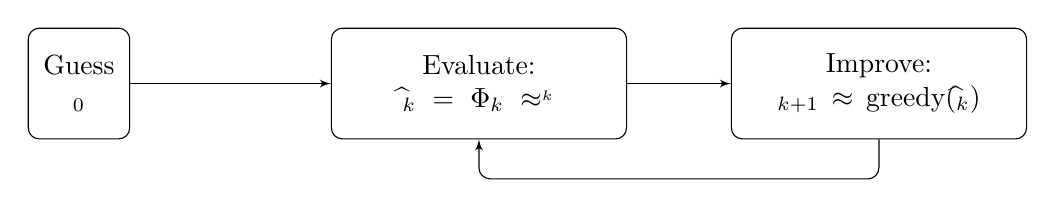
\begin{tikzpicture}[node distance = 2cm, auto]
    % Place nodes
    \node [block, node distance=1.5in, text width=3em] (a) {Guess $\policy_0$};
    \node [block, node distance=2in, right of =a, text width=10em] (b) {Evaluate: \\ $\widehat{\Value}_k=\FtrMtx \weights_k \approx \Value^{\policy_{k}}$ };
    \node [block, node distance=2in, right of = b, text width=10em] (c) {Improve: $\policy_{k+1}\approx \textrm{greedy}(\widehat{\Value}_k)$};
    % Draw edges
    \path [line] (a) -- (b);
    \path [line] (b) -- (c);
    \path [line,rounded corners] (c) |- ($(b.south east) + (0.5,-0.5)$) -| (b);
\end{tikzpicture}
\vspace{20pt}

A key question in approximate policy iteration, is how errors in the value-function approximation, and possibly also errors in the greedy policy update, affect the error in the final policy. The next result shows that if we can guarantee that the approximation errors are bounded at each step of the algorithm, then the error in the final policy will also be bounded. This result suggests that approximate policy iteration is a fundamentally sound idea.

\begin{theorem}\label{thm:API}
If for each iteration $k$ the policies are approximated well over $\States$:
\begin{equation}\label{eq:approx_pi_1}
\|\widehat{\Value}_k(\state)-\Value^{\policy_k}(\state)\|_\infty \le \delta,
\end{equation}
and policy improvement approximates well
\begin{equation}\label{eq:approx_pi_2}
\|\operator^{\policy_{k+1}}\widehat{\Value}_k - \operator\widehat{\Value}_k\|_\infty < \varepsilon,
\end{equation}
Then
$$ \limsup_k \ \| \Value^{\policy_k}(\state)-\Value^*(\state)\|_\infty \le \frac{\varepsilon+2\gamma\delta}{(1-\gamma)^2}.$$
\end{theorem}
\sloppy To understand the policy improvement approximation term \eqref{eq:approx_pi_2}, recall that the Bellman operator $\operator\widehat{\Value}_k$ corresponds to a greedy policy improvement step, $\policy_{\textrm{greedy}}\left(\widehat{\Value}_k\right)(\state) = \argmax_{\action} \reward(\state,\action) + \discount \sum_{\state'} \transitionprob(\state'|\state,\action)\widehat{\Value}_k(\state')$. Suppose we cannot perform the $\argmax$ accurately for every state when computing the next policy $\policy_{k+1}$, that is, $\policy_{k+1} \neq \policy_{\textrm{greedy}}\left(\widehat{\Value}_k\right)$. The condition \eqref{eq:approx_pi_2} ensures that $\policy_{k+1}$ is not too far off, in that $\reward(\state,\policy_{k+1}(\state)) + \discount \sum_{\state'} \transitionprob(\state'|\state,\policy_{k+1}(\state))\widehat{\Value}_k(\state')$ is not more than $\varepsilon$ away from $\policy_{\textrm{greedy}}\left(\widehat{\Value}_k\right)(\state)$.
\begin{proof}
    Let $e$ denote a vector of ones. From the contraction property of $\operator$ and $\operator^{\policy_{k+1}}$ we have that
    \begin{equation*}
        \| \operator^{\policy_{k+1}} \widehat{\Value}_k - \operator^{\policy_{k+1}}\Value^{\policy_k} \|_\infty \leq \discount \delta,
    \end{equation*}
    \begin{equation*}
        \| \operator \widehat{\Value}_k - \operator\Value^{\policy_k} \|_\infty \leq \discount \delta.
    \end{equation*}
    Therefore, 

    \begin{equation}\label{eq:approx_pi_3}
        \operator^{\policy_{k+1}}\Value^{\policy_k} \geq \operator^{\policy_{k+1}}\widehat{\Value}_k - \discount \delta e \geq \operator\widehat{\Value}_k - (\varepsilon + \discount \delta) e \geq \operator\Value^{\policy_k} - (\varepsilon + 2 \discount \delta) e
    \end{equation}
    where the inequalities are element-wise, the first inequality is by \eqref{eq:approx_pi_3}, the second inequality is by \eqref{eq:approx_pi_2}, and the last inequality is again by \eqref{eq:approx_pi_3}.
    Now, by definition of $\operator$,
    \begin{equation*}
        \operator\Value^{\policy_k} - (\varepsilon + 2 \discount \delta) e \geq \operator^{\policy_k}\Value^{\policy_k} - (\varepsilon + 2 \discount \delta) e = \Value^{\policy_k} - (\varepsilon + 2 \discount \delta) e,
    \end{equation*}
    so we have
    \begin{equation}\label{eq:approx_pi_4}
        \operator^{\policy_{k+1}}\Value^{\policy_k} \geq \Value^{\policy_k} - (\varepsilon + 2 \discount \delta) e.
    \end{equation}
    Since $\operator^{\policy_{k+1}}$ is a contraction and linear, we have that for any $\Value$ and a scalar $\alpha > 0$,
    \begin{equation*}
        \| \operator^{\policy_{k+1}}(\Value - \alpha e) - \operator^{\policy_{k+1}}\Value \|_\infty \leq \discount \alpha \| e \|_\infty = \discount \alpha.
    \end{equation*}
    Therefore, 
    \begin{equation}\label{eq:approx_pi_5}
        \operator^{\policy_{k+1}}(\Value - \alpha e) \geq \operator^{\policy_{k+1}}\Value - \discount \alpha e,
    \end{equation}
    and
    \begin{equation}\label{eq:approx_pi_5b}
        \operator^{\policy_{k+1}}(\Value - \alpha e) \leq \operator^{\policy_{k+1}}\Value + \discount \alpha e.
    \end{equation}
    Recalling that $\operator^{\policy_{k+1}}$ is a monotone operator (see proof of Lemma \ref{lemma:policy_improvement}), applying $\operator^{\policy_{k+1}}$ to both sides of \eqref{eq:approx_pi_4} and using \eqref{eq:approx_pi_5} we obtain:
    \begin{equation*}
    \left(\operator^{\policy_{k+1}}\right)^2\Value^{\policy_k} \geq \operator^{\policy_{k+1}}\Value^{\policy_k} - \discount(\varepsilon + 2 \discount \delta) e.
    \end{equation*}
    Similarly, applying $\left(\operator^{\policy_{k+1}}\right)^m$ to both sides of \eqref{eq:approx_pi_4} gives
    \begin{equation}\label{eq:approx_pi_6}
    \left(\operator^{\policy_{k+1}}\right)^{m+1}\Value^{\policy_k} \geq \left(\operator^{\policy_{k+1}}\right)^m\Value^{\policy_k} - \discount^m(\varepsilon + 2 \discount \delta) e.
    \end{equation}
    Now, consider the telescoping sum 
    \begin{equation*}    \left(\operator^{\policy_{k+1}}\right)^{n}\Value^{\policy_k} - \Value^{\policy_k} = \sum_{m=0}^{n-1}\left(\operator^{\policy_{k+1}}\right)^{m+1}\Value^{\policy_k} - \left(\operator^{\policy_{k+1}}\right)^m\Value^{\policy_k} \geq \left(\sum_{m=0}^{n-1}\discount^m\right)(\varepsilon + 2 \discount \delta) e,
    \end{equation*}
    where in the last equality we plugged \eqref{eq:approx_pi_6}. Taking $n \to \infty$ we obtain:
    \begin{equation}\label{eq:approx_pi_7}
        \Value^{\policy_{k+1}} - \Value^{\policy_k} \geq \frac{\varepsilon + 2 \discount \delta}{1 - \discount}e.
    \end{equation}
    Now,
    \begin{equation*}
    \begin{split}
        -\Value^{\policy_{k+1}} = -\operator^{\policy_{k+1}}\Value^{\policy_{k+1}} &= -\operator^{\policy_{k+1}}\Value^{\policy_{k}} - \left( \operator^{\policy_{k+1}}\Value^{\policy_{k+1}} - \operator^{\policy_{k+1}}\Value^{\policy_{k}}\right) \\ 
        &\leq -\operator^{\policy_{k+1}}\left(\Value^{\policy_{k}} + \frac{\varepsilon + 2 \discount \delta}{1 - \discount}e \right)\\
        &= \operator^{\policy_{k+1}}\left(-\Value^{\policy_{k}} - \frac{\varepsilon + 2 \discount \delta}{1 - \discount}e \right)\\
        &\leq -\operator^{\policy_{k+1}}\Value^{\policy_{k}} + \discount \frac{\varepsilon + 2 \discount \delta}{1 - \discount}e,
    \end{split}
    \end{equation*}
    where the first inequality is by \eqref{eq:approx_pi_7} and the second is by \eqref{eq:approx_pi_5b}.

    We next have,
    \begin{equation}\label{eq:approx_pi_8}
        \Value^{*} - \Value^{\policy_{k+1}} \leq \Value^{*} -\operator^{\policy_{k+1}}\Value^{\policy_{k}} + \discount \frac{\varepsilon + 2 \discount \delta}{1 - \discount}e.
    \end{equation}
    From the contraction of $\operator$ we have:
    \begin{equation}\label{eq:approx_pi_contraction}
        \Value^{*} - \operator \Value^{\policy_{k}} = \operator\Value^{*} - \operator \Value^{\policy_{k}} \leq \discount \|\Value^{*} - \Value^{\policy_{k}}\|_\infty e.
    \end{equation}
    From \eqref{eq:approx_pi_3}, we have
    \begin{equation*}
    \begin{split}
        \Value^{*} -\operator^{\policy_{k+1}}\Value^{\policy_{k}} &\leq \Value^{*} - \operator\Value^{\policy_k} + (\varepsilon + 2 \discount \delta) e \\
        &\leq \left(\discount \|\Value^{*} - \Value^{\policy_{k}}\|_\infty + \varepsilon + 2 \discount \delta\right)e
    \end{split}
    \end{equation*}
    Combining this with \eqref{eq:approx_pi_8} we obtain
    \begin{equation*}
        \Value^{*} - \Value^{\policy_{k+1}} \leq \left(\discount \frac{\varepsilon + 2 \discount \delta}{1 - \discount} + \discount \|\Value^{*} - \Value^{\policy_{k}}\|_\infty + \varepsilon + 2 \discount \delta\right)e = \left(\discount \|\Value^{*} - \Value^{\policy_{k}}\|_\infty + \frac{\varepsilon + 2 \discount \delta}{1 - \discount} \right)e.
    \end{equation*}
    Since by definition $\Value^{*} \geq \Value^{\policy_{k+1}}$, we must have
    \begin{equation*}
        \|\Value^{*} - \Value^{\policy_{k+1}}\|_\infty \leq \discount \|\Value^{*} - \Value^{\policy_{k}}\|_\infty + \frac{\varepsilon + 2 \discount \delta}{1 - \discount}.
    \end{equation*}
    The above holds for every $k$. Taking the $ \limsup$ of both sides as $k \to \infty$ (note that the policies and values do not necessarily converge, but $ \limsup$ always exists) we obtain,
    \begin{equation*}
        (1-\discount)\limsup_k\|\Value^{*} - \Value^{\policy_{k}}\|_\infty \leq  \frac{\varepsilon + 2 \discount \delta}{1 - \discount}.
    \end{equation*}
\end{proof}

\subsection{Approximate Policy Iteration Algorithms}

We next discuss several algorithms that implement approximate policy iteration. That is, methods for approximating the policy evaluation and the greedy policy improvement. We begin with methods that require knowledge of the state transition probabilities $\transitionkernel$, or a simulator thereof. We shall later consider methods that only require state transition samples.

\subsubsection{Classification Based Policy Iteration}
We have already discussed approximate policy evaluation in Section \ref{sec:approx_policy_eval}, so let us begin by assuming we have obtained an approximate value function $\widehat{\Value}^{\policy}(\state,\weights)$ for our current policy $\policy$. The main question is how obtain an (approximately) greedy policy $\policy_{\textrm{greedy}}\left(\widehat{\Value}^\policy\right)$ when the state space is too large to iterate over. We would like to treat this as another supervised learning problem. Therefore, we should
generate a training set, 
\[
D = \{(\state_1, \action_{\textrm{greedy}}(\state_1)),\ldots,
(\state_m,\action_{\textrm{greedy}}(\state_m))\},
\]
where the label of a sample state $\state$, $\action_{\textrm{greedy}}(\state)$, is an action taken from the greedy policy with resect to $\widehat{\Value}^{\policy}(\state,\weights)$.

We can use this training set to train a machine learning model for the greedy policy using standard supervised learning techniques, i.e., classification if the action space is finite or regression if the action space is continuous.
For concreteness, we focus here on a simple parametric method for finite actions; this approach extends naturally to other supervised learning techniques, including neural networks and non-parametric methods.
Let $\widehat{\policy}(\action | \state; \weights')$ be a policy parametrized by a weight vector $\weights'$ as follows,
\begin{equation*}
    \widehat{\policy}(\action | \state; \weights') = \frac{e^{\weight'^T \ftrs(\state,\action)}}{\sum_{\action'\in\Actions}e^{\weight'^T \ftrs(\state,\action')}},
\end{equation*}
where $\ftrs(\state,\action)$ are some state-action features (cf. the approximate $\QValue$ function in Section \ref{ssec:value_func_approx_arch}).
Note the distinction between the value function parameters $\weights$ and policy parameters $\weights'$. A standard classification technique for fitting the policy $\widehat{\policy}(\action | \state; \weights')$ to the data $D$ is maximum likelihood:
\begin{equation*}
    \weight'_{\textrm{ML}} = \argmax_{\weight'} \sum_{(\state_i, \action_{\textrm{greedy}}(\state_i)) \in D} \log \widehat{\policy}(\action_{\textrm{greedy}}(\state_i)) | \state_i; \weights'),
\end{equation*}
where the optimization is typically solved using gradient descent methods.

\begin{algorithm}[H]
\caption{Classification Based Approximate Policy Iteration}\label{alg:CB_API}
\begin{algorithmic}[1]
\State \textbf{Input:} Model $\transitionkernel$, policy $\policy_0$, size $N$, approximation architectures $\widehat{\Value}(\state, \weights)$, $\widehat{\policy}(\action | \state; \weights')$
\State \textbf{For} {$k = 0,1,2,\dots$ }
\State \quad Collect a set of $N$ samples $\{(\state_\ttime, \action_\ttime, \reward_\ttime, \state_{\ttime+1})\}$ under $\policy_k$
\State \quad \label{line:value_fit}Fit value function parameters $\weights_k$ 
\State \quad \label{line:label_generation}For each sample $\state_\ttime$ calculate
$$\action_{\textrm{greedy}}(\state_\ttime) = \argmax_{\action} \left\{\reward(\state_\ttime,\action) + \discount \sum_{\state'} \transitionprob(\state'|\state_\ttime,\action)\widehat{\Value}(\state', \weights_k)\right\}$$
\State \quad \label{line:policy_fit}Fit policy parameters $\weights'_k$
\begin{equation*}
    \weight'_k = \argmax_{\weight'} \sum_{(\state_\ttime, \action_{\textrm{greedy}}(\state_\ttime))} \log \widehat{\policy}(\action_{\textrm{greedy}}(\state_\ttime)) | \state_\ttime; \weights')
\end{equation*}
\end{algorithmic}
\end{algorithm}

Algorithm \ref{alg:CB_API} gives a template for classification-based approximate policy iteration. For the policy evaluation in Line \ref{line:value_fit}, any approximate policy evaluation method from Section \ref{sec:approx_policy_eval} can be used. The maximum-likelihood fit in Line \ref{line:policy_fit} can be replaced with different supervised learning methods for fitting a policy to data.
Note that we require the state transition probabilities $\transitionkernel$ for generating the greedy action labels in Line \ref{line:label_generation}. 

\subsubsection{Approximate Policy Iteration with $\tHorizon$-step Lookahead}

As long as we are generating improved actions for fitting the policy, there is no reason to limit ourselves to greedy actions. We can, for instance, calculate actions that are optimal with respect to a $\tHorizon$-step lookahead (whereas greedy corresponds to $\tHorizon=1$),

\begin{equation}\label{eq:lookahead_greedy}
    \policy_{\tHorizon-\textrm{greedy}}(\state_\ttime) = \argmax_{\action_\ttime} \left\{\max_{\policy}  \mathbb{E}^{\policy,\action_\ttime} \left[\sum_{\ttime'=\ttime}^{\ttime+\tHorizon-1} \discount^{\ttime' - \ttime}\reward(\state_{\ttime'}) + \discount^\tHorizon \widehat{\Value}(\state_{\ttime+\tHorizon}))\right]\right\}.
\end{equation}

The next theorem show that as we increase the lookahead horizon $\tHorizon$, the error bound for approximate policy iteration improves.

\begin{theorem}\label{thm:lookahead_API}
If for each iteration $k$ the policies are approximated well over $\States$:
\begin{equation}\label{eq:lookahead_approx_pi_1}
\|\widehat{\Value}_k(\state)-\Value^{\policy_k}(\state)\|_\infty \le \delta,
\end{equation}
and policy improvement approximates well
\begin{equation}\label{eq:lookahead_approx_pi_2}
\|\operator^{\policy_{k+1}}\widehat{\Value}_k - \operator^\tHorizon\widehat{\Value}_k\|_\infty < \varepsilon,
\end{equation}
Then
$$ \limsup_k \ \| \Value^{\policy_k}(\state)-\Value^*(\state)\|_\infty \le \frac{\varepsilon+2\gamma\delta}{(1-\gamma)(1-\gamma^\tHorizon)}.$$
\end{theorem}
\begin{proof}
    (Sketch) The proof follows the lines of Theorem \ref{thm:API}, where in Equation \ref{eq:approx_pi_contraction} we replace the $\discount$-contraction of $\operator$ with the $\discount^\tHorizon$ contraction of $\operator^\tHorizon$.
\end{proof}

Calculating the optimal action for a $\tHorizon$-step lookahead in \eqref{eq:lookahead_greedy} is not trivial for $\tHorizon > 1$, as essentially we need to solve a finite horizon MDP on a potentially large state space. Even if the number of possible state transitions for each state-action pair is bounded by some $M$, the number of states reachable from $\state_\ttime$ in $\tHorizon$ steps is bounded by $(\Actions M)^\tHorizon$, therefore searching for an optimal policy becomes intractable. 

A family of methods that has proven to work very well in practice approximates the optimal action in \eqref{eq:lookahead_approx_pi_2} using an approximate tree search algorithm. In particular, we focus here on the Monte-Carlo Tree Search (MCTS) algorithm.

\paragraph{Monte-Carlo Tree Search}
We can think of the optimization problem in \eqref{eq:lookahead_greedy} as finding an optimal action for each possible state that can be reached from $\state_\ttime$ in $\tHorizon$ steps. 

In MCTS, we sequentially build a tree representing the reachable states and their $\QValue$ values. The idea is to build the tree in a way that will focus on the more promising actions, and therefore will provide a good approximation of \eqref{eq:lookahead_approx_pi_2} even before the full tree is built. To do this, for each state we encounter, we maintain a $\QValue$ value estimate, and expand the tree sequentially by selecting actions that maximize, 
\begin{equation*}
    \action = \argmax \QValue(\state, \action) + B(\state,\action),
\end{equation*}
where $B(\state,\action)$ is an exploration bonus. Thus, most of the search is focused on exploring actions with a high $\QValue$ estimate, while the bonus term drives exploration of other actions, which is important in case the $\QValue$ estimate is not accurate.

A common term for the exploration bonus is termed \textit{upper confidence trees (UCT)},
\begin{equation*}
    B_{\textrm{UCT}}(\state,\action) = \frac{\sqrt{\log\sum_{\action'} N(\state,\action')}}{1+N(\state,\action)},
\end{equation*}
where $N(\state,\action)$ counts how many times a state-action pair was encountered during the tree search, and $\policy$ is the current policy in the approximate policy iteration. This term gives a higher bonus to actions that were not sampled often. Some motivation for this specific form of exploration-exploitation balance comes from a formal result that we shall establish in Chapter \ref{chapter:MAB} for the upper confidence bound algorithm. 

An alternative heuristic for the exploration bonus that was suggested in the popular Alpha Zero study takes into account the policy, and uses it to weigh the bonus term, 
\begin{equation*}
    B_{\textrm{AlphaZero}}(\state,\action) = \policy(\state,\action)\frac{\sqrt{\sum_{\action'} N(\state,\action')}}{1+N(\state,\action)}.
\end{equation*}

\begin{algorithm}[H]
\caption{Monte-Carlo Tree Search (MCTS)}\label{alg:MCTS}
\begin{algorithmic}[1]
\State \textbf{Input:} Simulator $\transitionkernel$, initial state $\state_{\textrm{root}}$, value estimate $\widehat{\Value}(\state)$, horizon $\tHorizon$, budget $K$
 \State Initialize Tree = $\{ \state_{\textrm{root}}\}$
 \State Initialize $\forall \action: \quad $ $W(\state_{\textrm{root}},\action) = 0$, $N(\state_{\textrm{root}},\action) = 0$, 
 $\QValue(\state_{\textrm{root}},\action) = 0$ 
 \State \textbf{For} {$k = 0,\dots,K$ }
 \State \quad \texttt{search}($\state$, 0)
 \State \textbf{Return} $\argmax_\action \QValue(\state_{\textrm{root}},\action)$
 \\
% \State Function{\texttt{search}}{$\state,\ttime$}
 \State 
 \textbf{function} \texttt{search}$(\state,\ttime)$
\State \quad \textbf{If} $\state \notin \textrm{Tree}$
\State \quad \quad Add $\state$ to Tree.
\State \quad \quad Initialize $\forall \action: \quad $ $W(\state,\action) = 0,$ 
$N(\state,\action) = 0,$ 
$\QValue(\state,\action) = 0$ 
\State \quad \quad \textbf{Return} $\widehat{\Value}(\state)$
\State \quad \textbf{If} $\ttime = \tHorizon$:
\State \quad \quad \textbf{Return} $\widehat{\Value}(\state)$
\State \quad $\action = \argmax \QValue(\state, \action) + B(\state,\action)$
\State \quad $\state' \sim \transitionprob(\cdot|\state,\action)$
\State \quad $W(\state,\action) = W(\state,\action) + \reward(\state,\action) + \discount\cdot$\texttt{search}($\state', \ttime+1$)
\State \quad $N(\state,\action) = N(\state,\action) + 1$
\State \quad $\QValue(\state, \action) = W(\state,\action) / N(\state,\action)$
\State \quad \textbf{Return} $\QValue(\state, \action)$
\end{algorithmic}
\end{algorithm}


Finally, we can use the MCTS algorithm \ref{alg:MCTS} as a replacement of the greedy action selection in Line \ref{line:label_generation} of the classification based approximate policy iteration algorithm \ref{alg:CB_API}, as an approximation of a $\tHorizon$-step lookahead action.

\begin{remark}
    In a very influential study~\cite{silver2017mastering}, a variant of the MCTS-based policy iteration algorithm above termed \emph{AlphaGo Zero} was used to train a super-human level policy in the challenging game of Go, and followup works extended the results to other board games~\cite{silver2018general}. These methods used deep neural networks for the policy and value function approximations, and were trained to play games using self-play: the policy was trained to play against itself as an opponent. For a fixed opponent policy, the game can be cast as an MDP as follows: following an action by the player at some state, the next state transition corresponds to first changing the board state according to the player's action, then using the policy to sample an action for the opponent, and subsequently changing board state according to the opponent action. In self-play, every once in a while, the opponent policy was changed to the currently trained policy, effectively changing the MDP.
\end{remark}

\subsubsection{Online Model Free Approximate Policy Iteration -- SARSA}

We now consider approximate policy iteration methods that do not require the model $\transitionkernel$ to compute the greedy improvement step. The main trick, similarly to the tabular setting, is to consider the state-action value function $\QValue$ instead of the state values $\Value$.

% As we have seen earlier, it is easier to define a policy improvement step using the $Q$ function. 

We start with an online method. For a given policy $\policy$, we can easily modify the TD(0) algorithm above to learn $\widehat{Q}^\policy(\state,\action;\weight)$.
% \begin{equation*}
%     \weights_{n+1} = \weights_n + \alpha_n \left( r(\state_n,a_n) + f(\state_{n+1},\action_{n+1};\weights_n) - f(\state_{n},\action_{n}; \weights_n) \right) \nabla_{\weights} f(\state_n,\action_n,\weights).
% \end{equation*}

\begin{algorithm}[H]
\begin{algorithmic}[1]
\State \textbf{Initialize:} Set $\weights_0 = 0$, $\state_0, \action_0$ arbitrary.
\State \textbf{For} {$\ttime = 0, 1, 2, \dots$}
    \State \quad Take action $\action_\ttime$ at state $\state_\ttime$
    \State \quad Observe $\reward_\ttime, \state_{\ttime+1}$
    \State \quad \label{line:sarsa_choose_action}Choose next action: $\action_{\ttime+1}$ 
    \State \quad Update:
  \[
    \weights_{\ttime+1} = \weights_\ttime + \alpha_\ttime \left( \reward(\state_\ttime,\action_\ttime) + \discount \widehat{Q}(\state_{\ttime+1},\action_{\ttime+1};\weights_\ttime) - \widehat{Q}(\state_{\ttime},\action_{\ttime}; \weights_\ttime) \right) \nabla_{\weights} \widehat{Q}(\state_\ttime,\action_\ttime; \weights_\ttime)\]
\end{algorithmic}
\caption{SARSA with Function Approximation}
\end{algorithm}


The actions in Line \ref{line:sarsa_choose_action} are typically selected according to an $\xi-$greedy or softmax rule. Thus, policy evaluation is interleaved with policy improvement.

\subsubsection{Batch Model Free Approximate Policy Iteration -- Least Squares Policy Iteration (LSPI)}
One can also derive an approximate policy iteration algorithm that works on a batch of data. Looking at the SARSA algorithm above, where action selection was updated throughout the run of the algorithm, this may seem a bit surprising -- how can we perform policy iteration on data that was collected once, using a single policy? The trick is to recall the Bellman equation for $\QValue$. Let $\policy_{\textrm{greedy}}$ be a policy that is greedy with respect to a value function $\widehat{Q}^\policy(\state,\action;\weight)$,  $\policy_{\textrm{greedy}}(\state) = \argmax_{\action}\widehat{Q}^\policy(\state,\action;\weight)$. Then $\QValue^{\policy_{\textrm{greedy}}}$ satisfies:
\begin{equation*}
\QValue^{\policy_{\textrm{greedy}}}(\state,\action) = \reward(\state,\action) + \discount \mathbb{E}\left[ \QValue^{\policy_{\textrm{greedy}}}(\state', \policy_{\textrm{greedy}}(\state'))\right].
\end{equation*}
Notice that in the equation above the expectation is with respect to the state transitions, and not any policy, therefore we can approximate it using a fixed set of samples. The Least Squares Policy Iteration (LSPI) builds on this idea to iteratively compute a least squares fit to the greedy policy with respect to the current $\QValue$.
Consider linear function approximation $\widehat{Q}^\policy(\state,\action) = \weights^T \ftrs(\state,\action)$. The idea is to use LSTD(0) to iteratively fit $\widehat{Q}^{\policy_k}$, where $\policy_k$ is the greedy policy w.r.t. $\widehat{Q}^{\policy_{k-1}}$.


\begin{algorithm}[H]
\caption{Least Squares Policy Iteration (LSPI)}
\begin{algorithmic}[1]
\State \textbf{Input:} Policy $\policy_0$
\State Collect a set of $N$ samples $\{(\state_\ttime, \action_\ttime, \reward_\ttime, \state_{\ttime+1})\}$ under $\policy_0$
\State \textbf{For} {$k = 1,2,\dots$ }
    \State \quad Compute: 
\begin{align*}
\widehat{A}_N^k &= \frac{1}{N} \sum_{\ttime=1}^N {\ftrs}(\state_\ttime,\action_\ttime)( {\ftrs}^T(\state_\ttime,\action_\ttime)-\gamma {\ftrs}^T(\state_{\ttime+1},\action^*_{\ttime+1})),
\end{align*}
\qquad where 
$\action^*_{\ttime+1} = \argmax_\action \widehat{Q}^{\policy_{k-1}}(\state_{\ttime+1},\action) = \argmax_\action \weights_{k-1}^T\ftrs(\state_{\ttime+1},\action)$
\begin{align*}
\widehat{b}_N^k &= \frac{1}{N} \sum_{\ttime=1}^N  {\ftrs}(\state_\ttime, \action_\ttime) \reward(\state_\ttime,\action_\ttime) 
\end{align*}
\State \quad Solve: 
\begin{align*}
\weights_k &= (\widehat{A}_N^k)^{-1} \widehat{b}_N^k
\end{align*}
\end{algorithmic}
\end{algorithm}

% \begin{align*}
% \widehat{b}_n^k &= \frac{1}{n} \sum_{\ttime=1}^n  {\ftrs}(\state_\ttime, \action_\ttime) \reward(\state_\ttime,\action_\ttime) 
% \end{align*}
% \begin{align*}
% \widehat{A}_n^k &= \frac{1}{n} \sum_{t=1}^n {\ftrs}(\state_\ttime,\action_\ttime)( {\ftrs}^T(\state_\ttime,\action_\ttime)-\gamma {\ftrs}^T(\state_{t+1},\action^*_{t+1})),
% \end{align*}
% \begin{align*}
% \weights_k &= (\widehat{A}_n^k)^{-1} \widehat{b}_n^k.
% \end{align*}
% where $\action^*_{t+1} = \argmax_\action \widehat{Q}^{\policy_{k-1}}(\state_{t+1},\action) = \argmax_\action \weights_{k-1}^T\ftrs(\state_{t+1},\action)$.

It is straightforward to extend the LSPI algorithm to nonlinear function approximation, by replacing LSTD with, e.g., projected value iteration (cf. Remark \ref{remark:non_linear_PVI}). It is also possible to collect data from the modified policy at each iteration $k$, instead of the initial policy.

\section{Approximate Value Iteration}
Approximate value iteration algorithms directly approximate the optimal value function (or optimal $Q$ function). Let us first consider the linear case. The idea in approximate VI is similar to the PBE, but replacing $\operator^\policy$ with $\operator^*$. That is, we seek solutions to the following projected equation:
\begin{equation*}
    \FtrMtx \weights = \Project \operator^* \{\FtrMtx \weights\},
\end{equation*}
where $\Project$ is some projection, such as the weighted least squares projection $\Project_\xi$ considered above. Recall that $\operator^*$ is a contraction in the $\|.\|_\infty$ norm. Unfortunately, $\Pi$ is not necessarily a contraction in $\|.\|_\infty$ for general function approximation, and not even for the weighted least squares projection $\Project_\xi$.\footnote{A restricted class of function approximators for which contraction does hold is called averagers, as was proposed in \cite{gordon1995stable}. The k-nearest neighbors approximation, for example, is an averager.} On the other hand, $\operator^*$ is not a contraction in the $\|.\|_\xi$ norm. Thus, we have no guarantee that the projected equation has a solution. Nevertheless, algorithms based on this approach have achieved impressive success in practice. 

% For the non-linear case, we have:
% \begin{equation*}
%     \widehat{Q}(\weights_{n+1}) = \Pi T \widehat{Q}(\weights_{n}).
% \end{equation*}

\subsubsection{Online Approximate Value Iteration -- Q Learning}
The function approximation version of online Q-learning resembles SARSA, only with an additional maximization over the next action:
% \begin{equation*}
%     \weights_{n+1} = \weights_n + \alpha_n \left( \reward(\state_n,\action_n) + \discount \max_\action \widehat{Q}(\state_{n+1},\action;\weights_n) - \widehat{Q}(\state_{n},\action_{n}; \weights_n) \right) \nabla_{\weights} \widehat{Q}(\state_n,\action_n,\weights).
% \end{equation*}

\begin{algorithm}[H]
\caption{Q-learning with Function Approximation}\label{alg:Q-learning}
\begin{algorithmic}[1]
\State \textbf{Initialize:} Set $\weights_0 = 0$.
\State \textbf{For} {$\ttime = 0, 1, 2, \dots$}
    \State \quad Observe: $\state_\ttime$ 
    \State \quad Choose action: $\action_\ttime$ 
    \State \quad Observe $\reward_\ttime, \state_{\ttime+1}$
    \State \quad Update:
    \begin{equation*}
    \weights_{\ttime+1} = \weights_\ttime + \alpha_\ttime \left( \reward(\state_\ttime,\action_\ttime) + \discount \max_\action \widehat{Q}(\state_{\ttime+1},\action;\weights_\ttime) - \widehat{Q}(\state_{\ttime},\action_{\ttime}; \weights_\ttime) \right) \nabla_{\weights} \widehat{Q}(\state_\ttime,\action_\ttime,\weights).
\end{equation*}
\end{algorithmic}
\end{algorithm}

The actions are typically selected according to an $\varepsilon-$greedy or softmax rule, to balance exploration and exploitation.

\subsubsection{Batch Approximate Value Iteration -- Fitted Q}

In this approach, we iteratively project (fit) the Q function based on the projected equation:
\begin{equation*}
    \widehat{Q}(\weights_{n+1}) = \Project \operator^* \widehat{Q}(\weights_{n}).
\end{equation*}

Assume we have a data set of samples $\{\state_i,\action_i,\state'_i,\reward_i\}$,obtained from some data collection policy. Then, the right hand side of the equation denotes a regression problem where the samples and labels are: $\left\{(\state_i,\action_i), \reward_i + \discount \max_\action \widehat{Q}(\state'_i, \action;\weights_{n})\right\}$. Thus, by solving a sequence of regression problems we approximate a solution to the projected equation.

\begin{algorithm}[H]
\caption{Fitted Q Learning}\label{alg:fitted_Q}
\begin{algorithmic}[1]
\State \textbf{Input:} Data collection policy $\policy_0$, approximation architecture $\widehat{Q}(\state, \action;\weights)$
\State Initialize $\weights_{0}=0$
\State Collect a set of $N$ samples $\{(\state_\ttime, \action_\ttime, \reward_\ttime, \state_{\ttime+1})\}$ under $\policy_0$
\State \textbf{For} {$k = 0,1,2,\dots$ }
    \State \quad Compute labels for each sample $x_\ttime = (\state_\ttime, \action_\ttime)$: 
\begin{align*}
y_\ttime = \reward_\ttime + \discount \max_\action \widehat{Q}(\state_{\ttime+1}, \action;\weights_{k})
\end{align*}
\State \quad Solve least-squares regression for $\{ (x_\ttime,y_\ttime)\}$: 
\begin{align*}
\weights_{k+1} &= \argmin_\weights \frac{1}{N}\sum_{\ttime} \left( \widehat{Q}(\state_{\ttime}, \action_\ttime;\weights) - y_\ttime\right)^2
\end{align*}
\end{algorithmic}
\end{algorithm}


Note that approximate VI algorithms are \emph{off-policy} algorithms. Thus, in both Q-learning and fitted-Q, the policy that explores the MDP can be arbitrary (assuming of course it explores `enough' interesting states).

\subsubsection{The Deep Q Learning Algorithm}

A notable milestone in RL history is the application of RL to a large collection of Atari games, using the Deep Q Learning (DQN) algorithm~\citep{mnih2015human}, which advanced the study of deep RL. DQN employed several  techniques to stabilize learning, which were important for its training with deep neural networks. Here, we shall see that these techniques resemble a mix of online Q learning and batch fitted Q.

\paragraph{Replay Buffer} The algorithm is online, similarly to the Q learning Algorithm \ref{alg:Q-learning}. However, instead of updating the $\QValue$ function weights using the current $(\state,\action,\reward,\state')$ sample, as in Q learning, the current sample is stored in a buffer, and a random sample is retrieved from the buffer to perform the update. This works to break correlations between subsequent updates to the $\QValue$ function, which may arise from the algorithm encountering similar states during the agent's interaction with the environment.

\paragraph{Target $\QValue$ Network} 
Similarly to the fitted Q algorithm \ref{alg:fitted_Q}, DQN uses the same weight vector $\bar{\weights}$ in the labels $\reward(\state_\ttime,\action_\ttime) + \discount \max_\action \widehat{Q}(\state_{\ttime+1},\action;\bar{\weights})$ for multiple updates of the algorithm. This works to stabilize the training, as current changes to the $\QValue$ approximation do not affect the update direction. Every fixed number of updates, the \textit{target} weights $\bar{\weights}$ are replaced to be the current weights.

\begin{algorithm}[H]
\caption{DQN}\label{alg:DQN}
\begin{algorithmic}[1]
\State \textbf{Input:} Replay buffer size $N$, initial weights, $\weights_0$, initial state $\state_0$, target update rate $K$, minibatch size $B$
\State \textbf{Initialize:} Set target weights $\bar{\weights} = \weights_0$, replay buffer $D = \{ \}$
\State \textbf{For} {$\ttime = 0, 1, 2, \dots$}
    \State \quad Observe: $\state_\ttime$ 
    \State \quad \label{line:dqn_action_selection}Choose action: $\action_\ttime$ 
    \State \quad Observe $\reward_\ttime, \state_{\ttime+1}$
    \State \quad Add $\left(\state_\ttime,  \action_\ttime, \reward_\ttime, \state_{\ttime+1}\right)$ to $D$
    \State \quad Sample minibatch $b = \left\{\left(\state_i,  \action_i, \reward_i, \state_{i}'\right)\right\}$ of size $B$ uniformly from $D$ 
    \State \quad Compute labels for each sample $x_i = (\state_i, \action_i)$ in $b$: 
\begin{align*}
y_i = \reward_i + \discount \max_\action \widehat{Q}(\state_{i}', \action;\bar{\weights})
\end{align*}
    \State \quad Take gradient descent step:
    \begin{equation*}
    \weights_{\ttime+1} = \weights_\ttime + \alpha_\ttime \nabla_{\weights} \left( \frac{1}{B}\sum_{(x_i,y_i)\in b} \left(\widehat{Q}(\state_{i}, \action_{i};\weights_\ttime) - y_i)\right)^2\right) 
\end{equation*}
\State \quad Every $K$ iteration set $\bar{\weights} = \weights_\ttime$
\end{algorithmic}
\end{algorithm}

As in the Q learning algorithm, action selection in Line \ref{line:dqn_action_selection} of DQN follows  an $\varepsilon-$greedy or softmax rule, to balance exploration and exploitation.

\section{Off-Policy Learning with Function Approximation (Yishay to Check)}
\label{sec:off_policy_FA}

We would like to see what is the effect that the samples are generated
following a different policy, namely, an off-policy setting. There
is no issue for Monte-Carlo, and the same logic would still be
valid.  For TD, we did not have any problem in the look-up model. We
would like to see what can go wrong when we have a function
approximation setting.


\begin{figure}
  % Requires \usepackage{graphicx}
  \begin{centering}
  \includegraphics[width=0.5\textwidth]{figures/L8-2states.png}\\
  \caption{Two state snippet of an MDP }\label{fig:L8-2state}
  \end{centering}
\end{figure}

Consider the following part of an MDP (see Figure
\ref{fig:L8-2state}) consists of two nodes, with a transition from
the first to the second, with reward $0$. The main issue is that the
linear approximation gives the first node a weight $\weight$ and the
second $2\weight$. Assume we start with some value $\weight_0>0$.
Each time we have an update for the two states we have
\[
\weight_{\ttime+1}=\weight_\ttime +\alpha[0+\gamma
(2\weight_\ttime)-\weight_\ttime]=[1+\alpha(2\gamma-1)]\weight_\ttime=[1+\alpha(2\gamma-1)]^\ttime\weight_1
\]
For $\gamma>0.5$ we have $\alpha(2\gamma-1)>0$, and $\weight_\ttime$
diverges.

We are implicitly assuming that the setting is off-policy, since in
an on-policy, we would continue from the second state, and
eventually lower the weight.

To have a ``complete'' example consider the three state MDP in
Figure~\ref{fig:L8-3state}. All the rewards are zero, and the main
difference is that we have a new terminating state, that we reach
with probability $p$.

\begin{figure}
  % Requires \usepackage{graphicx}
  \begin{centering}
  \includegraphics[width=0.5\textwidth]{figures/L8-3state.png}\\
  \caption{The three state MDP. All rewards are zero.}\label{fig:L8-3state}
  \end{centering}
\end{figure}




Again, assume that we start with some $\weight_0>0$ We have three
types of updates, one per possible transition. When we transition
from the initial state to the second state we have
\[
\Delta \weight= \alpha[0+\gamma
(2\weight_\ttime)-\weight_\ttime]\cdot
1=\alpha(2\gamma-1)\weight_\ttime
\]
The transition from the second state back to itself has an update,
\[
\Delta \weight= \alpha[0+\gamma
(2\weight_\ttime)-(2\weight_\ttime)]\cdot 2
=-4\alpha(1-\gamma)\weight_\ttime
\]
The transition to the terminal state we have
\[
\Delta \weight= \alpha[0+\gamma 0 -(2\weight_\ttime)]\cdot
2=-4\alpha \weight_\ttime
\]



When we use on-policy, we have all transitions. Assume that the
second transition happens $n\geq 0$ times. Then we have
\[
\frac{\weight_{\ttime+1}}{\weight_\ttime}=(1+\alpha(2\gamma-1))(1-4\alpha(1-\gamma))^n(1-4\alpha)<
1-\alpha
\]
This implies that $\weight_\ttime$ converges to zero, as desired.

Now consider an off-policy that truncates the episodes after $n$
transitions of the second state, where $n\ll 1/p$, and in addition
$\gamma> 1-1/(40n)$. This implies that in most updates we do not
reach the terminal state and we have
\[
\frac{\weight_{\ttime+1}}{\weight_\ttime}=(1+\alpha(2\gamma-1))(1-4\alpha(1-\gamma))^n>1
\]
and therefore, for some setting of $n$ we have that the weight
$\weight_\ttime$ diverges.

We might hope that the divergence is due to the online nature of the
TD updates. We can consider an algorithm that in each iteration
minimizes the square error. Namely,
\[
\weight_{\ttime+1}=\arg\min_\weight\sum_s
[\widehat{\Value}(\state_\ttime;\weight)-E^\policy[\reward_\ttime+\gamma\widehat{\Value}(\state_{\ttime+1};\weight_\ttime)]]^2
\]

For the MDP example of Figure~\ref{fig:L8-3state} we have that:
\begin{align*}
 \weight_{\ttime+1} &= \arg\min_\weight (\weight-\gamma(2\weight_\ttime))^2+(2\weight-(1-p)\gamma(2\weight_\ttime))^2
\end{align*}
Solving for $\weight_{\ttime+1}$ we have
\begin{align*}
0&=  2(\weight_{\ttime+1}-\gamma(2\weight_\ttime))+4(2\weight_{\ttime+1}-(1-p)\gamma(2\weight_\ttime)\\
  10 \weight_{\ttime+1}&=4\gamma \weight_\ttime + 8\gamma(1-p)\weight_\ttime\\
  \weight_{\ttime+1}&=\frac{6-4p}{5}\gamma \weight_\ttime
\end{align*}
So for $\gamma(6-4p)>5$ we have divergence. (Recall that
$\gamma\approx 1-\varepsilon$ and $p\approx \varepsilon$ is a very
important setting.\AT{what is $\varepsilon$ here?})

Note that if we have taken in to account the influence of
$\weight_{\ttime+1}$ on $\Value$ and use
$\widehat{\Value}(\state_{\ttime+1};\weight_{\ttime+1})$ instead of
$\widehat{\Value}(\state_{\ttime+1};\weight_\ttime)$, this specific
problem would have disappeared, since $\weight_{\ttime+1}=0$ would
be the minimizer.

\subsubsection{Summary of convergence results} Here is a summary of the known convergence and divergence results in
the literature:
\begin{center}
  \begin{tabular}{ | l | c | c|c|c| }
    \hline
    & algorithm & look-up table&linear function&non-linear\\ \hline
    on-policy & MC & + & + & + \\ \hline
    on-policy & $TD(0),TD(\lambda)$ & + & + & -\\ \hline
 %   on-policy & $TD(\lambda)$ & + & + & - \\ \hline
    off-policy & MC & + & + & + \\ \hline
    off-policy & $TD(0),TD(\lambda)$ & + & - & -\\ \hline
 %   off-policy & $TD(\lambda)$ & + & - & - \\ \hline
  \end{tabular}
\end{center}

The results for the look-up table where derived in Chapter
\ref{chapter:learning-model-free}.
%
The fact that Monte-Carlo methods converge is due to the fact that
they are running an SGD algorithm. For linear functions with convex
loss they will converge to the global optimum and for non-linear
functions (for example, neural networks) they will converge to a
local optima. The convergence to the TD appear in Chapter
\ref{ssec:TD_solution_techniques}. The divergence of TD with linear functions in
an off-policy setting appear in Chapter \ref{sec:off_policy_FA}. The TD
divergence in the non-linear online setting appears in
\cite{TsitsiklisVR97}.


\section{Bibliography Notes}
The idea of using function approximation for value functions dates back to the previous century \cite{bellman1959functional,shannon1950xxii,barto1983neuronlike,Tesauro02}.
The error bounds for approximate value iteration and approximate policy iteration presented here were developed in \cite{BertsekasTsitsiklis96}. Error bounds based on the L$2$ norm were developed by Munos \citep{munos2007performance}.

Least squares regression is a standard statistical method in machine learning~\citep{mohri2018foundations,shalev2014understanding}.

The projected Bellman equation and its analysis can be found in \citep{Bertsekas05}.
The LSTD algorithm is due to \cite{bradtke1996linear}, and was further investigated in \cite{boyan2002technical}. The LSPI algorithm is by \citep{lagoudakis2003least}. Fitted Q learning and approximate value iteration was proposed in several different studies \citep{gordon1995stable, tsitsiklis1996feature, riedmiller2005neural, ormoneit2002kernel, ernst2005approximate}. The deep Q learning algorithm is by \citep{mnih2015human}.
The convergence of TD(0) with linear function approximation was established in \citep{tsitsiklis1996analysis}.
Classification based policy iteration was studied in \cite{lagoudakis2003reinforcement,lazaric2010analysis,scherrer2015approximate}. Approximate PI with multi-step lookahead was proposed in \citep{efroni2018beyond}. 

Monte Carlo Tree Search was developed by \citep{coulom2006efficient,kocsis2006bandit}. Its extension using RL was applied to Go and other board games by \citep{silver2016mastering,silver2018general}.